\documentclass{article}

% NeurIPS 2026 style (default = main track, double-blind)
\usepackage{neurips_2026}

% Common packages
\usepackage[utf8]{inputenc}
\usepackage[T1]{fontenc}
\usepackage{hyperref}
\usepackage{url}
\usepackage{booktabs}
\usepackage{amsfonts}
\usepackage{nicefrac}
\usepackage{microtype}
\usepackage{xcolor}
\usepackage{bbm}
% Additional packages from the ICML version
\usepackage{graphicx}
\usepackage{subcaption}
\usepackage{multirow}
\usepackage{tabularx}
\usepackage{threeparttable}
\usepackage{amsmath}
\usepackage{amssymb}
\usepackage{mathtools}
\usepackage{amsthm}
\usepackage{pifont}

% Plotting
\usepackage{tikz}
\usepackage{pgfplots}
\pgfplotsset{compat=1.18}

% cleveref (load after hyperref)
\usepackage[capitalize,noabbrev]{cleveref}

%%%%%%%%%%%%%%%%%%%%%%%%%%%%%%%%
% THEOREMS
%%%%%%%%%%%%%%%%%%%%%%%%%%%%%%%%
\theoremstyle{plain}
\newtheorem{theorem}{Theorem}[section]
\newtheorem{proposition}[theorem]{Proposition}
\newtheorem{lemma}[theorem]{Lemma}
\newtheorem{corollary}[theorem]{Corollary}
\theoremstyle{definition}
\newtheorem{definition}[theorem]{Definition}
\newtheorem{assumption}[theorem]{Assumption}
\theoremstyle{remark}
\newtheorem{remark}[theorem]{Remark}

\title{Scaling ANN-to-SNN Conversion to Large Language Models via Representation and Local Approximation}

% Anonymized for double-blind review
\author{Anonymous Authors \\
Paper under double-blind review}

\begin{document}

\maketitle

\begin{abstract}
% ANN-to-SNN conversion has stalled at large language model (LLM) scale: prior
% methods report double-digit perplexity degradations on billion-parameter
% transformers, and the underlying mechanism is clear---per-layer conversion
% error compounds through depth, and in a 32--80 block transformer the compounded
% error is severe enough to render the converted model unusable. We identify a
% structural fix and demonstrate that it clears this bottleneck empirically.

% The fix comes from reframing conversion as a \emph{representation} problem
% rather than an approximation problem. An $N$-bit quantized value already has a
% finite, exact representation---its binary expansion---so a spike train of
% length $N$ can carry it without loss. \textbf{Bit Spike Encoding (BSE)}
% realizes this: a positional-threshold integrate-and-fire neuron produces a
% bijective map between $N$-bit quantized values and $N$-timestep spike trains,
% and under calibration alignment with the ANN's quantization grid, every linear
% layer in the SNN is \emph{functionally identical} to its $N$-bit quantized ANN
% counterpart. The conversion problem thereby reduces to the quantization
% problem for linear layers, leaving only nonlinear activations as irreducible
% approximation sites; \textbf{Adaptive Spiking Neural Codec (ASNC)} handles
% these via distribution-aware piecewise adaptation with BSE re-encoding at the
% output, localizing the remaining approximation error at each nonlinear site
% rather than diffusing it layer-wise.

% Empirically, LASER is the first method we are aware of to convert LLMs up to
% 70B parameters under an FP16/16-step regime with $<\!2\%$ accuracy degradation
% across MMLU, HellaSwag, ARC, and TruthfulQA. The degradation does not grow
% systematically across a panel of five transformers spanning 32 to 80 blocks,
% which is consistent with the error localization predicted by our analysis.
% Controlled internal baselines confirm that both BSE and ASNC are necessary;
% external comparison to prior SNN work is deliberately scoped as cross-regime
% because no prior method has reported matched FP16/16-step numbers at this
% scale (this absence is itself evidence of the bottleneck). On Intel Loihi~2,
% a single ASNC nonlinear operation consumes $\approx\!0.5\%$ of the equivalent
% GPU energy ($>\!200\times$ reduction at the component level); full-model
% neuromorphic inference awaits hardware support for the BSE linear and DCR
% paths and is out of scope here.

ANN-to-SNN conversion has struggled at large language model (LLM) scale, where prior methods exhibit severe degradation due to error accumulation across deep transformer stacks. We identify the root cause as structural: existing approaches treat conversion as a layer-wise approximation problem, causing errors to compound with depth.
%
We instead decompose conversion into representation and approximation. Bit Spike Encoding (BSE) provides a bijective mapping between quantized values and spike trains, enabling linear layers to be computed exactly relative to their quantized ANN counterparts, without introducing additional conversion error. This reduces the problem to nonlinearities, which are the only remaining approximation sites. We address these with Adaptive Spiking Neural Codec (ASNC), a distribution-aware piecewise scheme that produces bounded approximation error and re-encodes outputs into the BSE format, thereby localizing error at each nonlinear module.
%
Under this formulation, we derive an end-to-end error bound showing that conversion error is governed by nonlinear modules and their Lipschitz properties, rather than by network depth. Empirically, LASER converts LLMs up to 70B parameters under an FP16/16-step regime with less 2\% degradation across MMLU, HellaSwag, ARC, and TruthfulQA, without degradation scaling across models from 32 to 80 transformer blocks.
\end{abstract}


\section{Introduction}
\label{sec:introduction}

Large language models are exactly the workload where neuromorphic hardware
would pay off most: billion-parameter transformers dominate inference energy
budgets, and event-driven substrates like Intel Loihi~2 offer order-of-magnitude
energy reductions if the model can be expressed as an
SNN~\citep{davies2018loihi,davies2021loihi}. Yet ANN-to-SNN conversion---the
natural route, since it preserves the capability learned during pretraining---%
has not crossed the threshold to LLM scale. Prior conversion methods report
perplexity degradations in the double digits on billion-parameter transformers,
or require timestep budgets of $10^3$ or more to approach acceptable
accuracy~\citep{xing2025spikellm,zhou2024spikformerv2,ZhaoHuangDingYu2025_TTFSFormer}.
Conversion for LLMs has been, in practical terms, an unsolved problem.

The mechanism is structural. Every existing conversion path introduces
approximation \emph{at every layer}: lossy spike encodings (rate coding,
TTFS) at every activation, architectural substitution at every
nonlinearity~\citep{zhou2023spikformer,yao2023sdt,spikedattention2024}, and
heuristic surrogate gradients at every backward
step~\citep{neftci2019surrogate,shrestha2018slayer,deng2022tet}. In a shallow
vision network these per-layer errors are manageable. In a transformer with
tens of layers they begin to accumulate; in a 32-block LLM they compound to
the point of failure; in a 70B-parameter 80-block model they saturate any
reasonable accuracy budget. The problem is not any individual conversion step, but the accumulation of error through depth, which LLMs are too deep to absorb.

The right place to intervene is the representation itself. Prior methods treat conversion as an \emph{approximation} problem: continuous values are approximated by discrete spike trains at every layer, and the resulting error accumulates through depth. While each approximation may be small, its repeated application leads to large degradation in deep models such as LLMs. The issue is therefore not any individual conversion step, but that approximation is introduced everywhere, causing total error to grow with model depth.
%
To address this, we reduce both the amount and the spread of approximation. An $N$-bit quantized value already admits an exact discrete representation—its binary expansion—and a spike train of length $N$ can encode it without loss. This allows linear layers to be implemented without introducing additional conversion error, reducing the linear path to standard quantized ANN computation. The remaining approximation is confined to nonlinear operations, which cannot be made exact in the discrete domain.

We realize this decomposition in LASER through two components. \textbf{Bit Spike Encoding (BSE)} provides a bijective mapping between $N$-bit quantized values and $N$-timestep spike trains, ensuring that linear layers match their quantized ANN counterparts. \textbf{Adaptive Spiking Neural Codec (ASNC)} handles nonlinearities with bounded, distribution-aware approximation and re-encodes outputs into the same representation, so that approximation error remains localized. As a result, total conversion error depends only on a small set of nonlinear modules, rather than accumulating across all layers, enabling stable conversion even in deep LLMs. Our main contribution are:
\begin{itemize}
  \item \textbf{Structural diagnosis.}
  We identify depth-wise error accumulation as the key limitation of prior ANN-to-SNN conversion methods at LLM scale, arising from approximation introduced at every layer.

  \item \textbf{Representation–approximation decomposition.}
  We propose a framework that eliminates approximation in linear layers via Bit Spike Encoding (BSE) and confines it to nonlinear operations via Adaptive Spiking Neural Codec (ASNC), reducing both the amount and spread of error.

  \item \textbf{End-to-end error analysis.}
  We show that, under this decomposition, total conversion error depends only on nonlinear modules and their Lipschitz properties, rather than accumulating across all layers.

  \item \textbf{LLM-scale empirical validation.}
  We demonstrate stable conversion of transformers up to 70B parameters under a 16-step regime, with minimal degradation and no systematic growth with model depth.
\end{itemize}

\section{Related Work}
\label{sec:related_works}

ANN-to-SNN conversion has been studied along three axes, each contributing its
own approximation errors.

\noindent\textbf{Spike encoding.}
Rate coding~\citep{rueckauer2017conversion,auge2021encoding,guo2021coding}
requires thousands of timesteps for acceptable precision; TTFS~%
\citep{bonilla2022ttfs,stanojevic2024ttfs} reduces latency at the cost of a
single-spike constraint, and TTFS-Former still requires 1{,}024 steps for FP16
precision~\citep{ZhaoHuangDingYu2025_TTFSFormer}. Spikformer and
Spikformer-v2~\citep{zhou2023spikformer,zhou2024spikformerv2} and
SpikeZIP-TF~\citep{you2024spikeziptf} trade latency for accuracy via long time
windows. All these schemes are lossy many-to-one mappings between continuous
values and spike trains. BSE differs fundamentally in being bijective: it
represents an $N$-bit integer by its binary expansion across $N$ timesteps, so
no information is lost in transit.

\noindent\textbf{Nonlinear computation.}
SiLU, Softmax, and LayerNorm have no exact spike-domain equivalent, forcing
either structural substitution---SSA in Spikformer~\citep{zhou2023spikformer},
rewrites in Spike-Driven
Transformer~\citep{yao2023sdt,spikedattention2024,wang2023stsa}---or
approximate equivalence~\citep{you2024spikeziptf,tang2024sorbet,zhu2023spikegpt,
xing2025spikellm}. Both paths inject per-site approximation errors. ASNC
differs from prior approximate approaches in two ways: it allocates segments
non-uniformly to match the empirical activation density, and its outputs are
re-encoded into BSE format so that downstream linear layers inherit the
BSE--quantized-ANN equivalence.

\noindent\textbf{Training.}
Surrogate gradients~\citep{neftci2019surrogate,wu2018stbp,shrestha2018slayer}
are the standard remedy for non-differentiable spikes, applied globally without
any guarantee of forward-backward consistency.
STBP~\citep{wu2018stbp}, SLAYER~\citep{shrestha2018slayer}, and
DIET-SNN~\citep{rathi2021dietsnn} reduce stability at scale; conversion with
fine-tuning~\citep{rathi2020hybrid} and direct training~\citep{xing2024spikelm}
share the same limitation. Our STE characterization under LASER is narrower in
scope: we do not claim an unconditional surrogate-gradient remedy, only that
under BSE and ASNC the forward-backward mismatch can be characterized
layer-type by layer-type rather than treated as a global heuristic.

% \noindent\textbf{Quantization and depth-aware bounds.}
% Our framework adopts tooling from the post-training and quantization-aware
% training works~\citep{nagel2020up,li2021brecq,nagel2021white,lin2024duquant,
% he2024understanding}. Activation calibration, per-channel affine ranges, and
% Lipschitz-chain error decomposition all have direct precedents there. The
% contribution of LASER is not a new analytical tool but the specific
% \emph{architectural reduction}: under BSE, the SNN forward pass is
% isomorphic to the quantized ANN forward pass modulo the ASNC nonlinear sites,
% which lets us import the quantization-literature bounds directly and concentrate
% SNN-specific analysis on the nonlinear modules.


%%%%%%%%%%%%%%%%%%%%%%%%%%%%%%%%%%%%%%%%%%%%%%%%%%%%%%%%%%%%%%%%%%%%%%%%%%%
\section{Preliminaries}
\label{sec:preliminaries}
%%%%%%%%%%%%%%%%%%%%%%%%%%%%%%%%%%%%%%%%%%%%%%%%%%%%%%%%%%%%%%%%%%%%%%%%%%%

\noindent\textbf{SNN Computation Model.}
We adopt the non-leaky Integrate-and-Fire (IF) model with soft reset and dynamic
threshold as the computational primitive. Given input current $I_{\mathrm{in}}(t)$,
membrane potential $V_m(t)$, and dynamic threshold $\Theta(t)$, the neuron emits
spike $S(t) \in \{0,1\}$ and updates via
\begin{equation}
\label{eq:if_forward}
S(t) = \mathbbm{1}\!\left[V_m(t) + I_{\mathrm{in}}(t) \ge \Theta(t)\right], \qquad
V_m(t{+}1) = V_m(t) + I_{\mathrm{in}}(t) - S(t)\,\Theta(t),
\end{equation}
initialized with $V_m(0) = 0$. 
For a layer of $d$ neurons, these updates apply elementwise, yielding
$\mathbf{S}(t) \in \{0,1\}^d$. A spiking layer maps an input spike
sequence to an output spike sequence via these dynamics, and stacking
such layers defines the network function $\mathcal{F}_{\mathrm{SNN}}$.
%
Setting $\Theta(t)$ to a fixed positional schedule
realizes BSE; making it learnable realizes ASNC. A layer's output is the spike
train $\mathbf{S} = (S(0), \dots, S(T-1)) \in \{0,1\}^T$.

\noindent\textbf{Formal Problem Statement.}
Let $\mathcal{F}_{\mathrm{ANN}}$ be a feedforward network alternating affine
operations $\mathbf{z}^\ell = \mathbf{W}^\ell \mathbf{x}^{\ell-1} + \mathbf{b}^\ell$
and nonlinearities $\mathbf{x}^\ell = \sigma(\mathbf{z}^\ell)$.
%
Let $\mathcal{F}_{\mathrm{QANN}}$ denote its $N$-bit quantized counterpart.
ANN-to-SNN conversion seeks a spiking network $\mathcal{F}_{\mathrm{SNN}}$
such that
\begin{equation}
\label{eq:conversion_goal}
\bigl\|\mathcal{F}_{\mathrm{SNN}}(\mathbf{x}^0)
      - \mathcal{F}_{\mathrm{QANN}}(\mathbf{x}^0)\bigr\|
\;\le\; \epsilon_{\mathrm{conv}},
\end{equation}
with all inter-layer communication realized via binary spike trains.
%
The total deviation from the full-precision ANN decomposes as
\[
\|\mathcal{F}_{\mathrm{SNN}}(\mathbf{x}^0)
- \mathcal{F}_{\mathrm{ANN}}(\mathbf{x}^0)\|
\;\le\;
\epsilon_{\mathrm{conv}} + \epsilon_{\mathrm{quant}},
\]
where $\epsilon_{\mathrm{quant}}$ is the quantization error.

\noindent\textbf{Worst-case conversion-error accumulation.}
Let $\mathbf{y}=\mathcal{F}_{\mathrm{QANN}}(\mathbf{x}^0)$ denote the
$N$-bit quantized ANN output and
$\hat{\mathbf{y}}=\mathcal{F}_{\mathrm{SNN}}(\mathbf{x}^0)$ its SNN counterpart.
Suppose layer $\ell$ introduces relative conversion error $\epsilon_\ell$, and
the nonlinearities are $L_\sigma$-Lipschitz. Then
\begin{equation}
\label{eq:error_accumulation}
\|\hat{\mathbf{y}}-\mathbf{y}\|
\;\le\;
\|\mathbf{y}\|\prod_{\ell=1}^{L}(1+L_\sigma\epsilon_\ell)
\;=\;
O\!\left((1+\epsilon)^L\right),
\end{equation}
where $\epsilon=\max_\ell \epsilon_\ell$.
This bound motivates LASER: if conversion error is eliminated for linear
layers and bounded only at nonlinear layers, then accumulation is governed
by the nonlinear modules rather than by all layers in the network. The total deviation from the full-precision ANN further decomposes into conversion error plus the fixed quantization floor.


%%%%%%%%%%%%%%%%%%%%%%%%%%%%%%%%%%%%%%%%%%%%%%%%%%%%%%%%%%%%%%%%%%%%%%%%%%%
\section{Methodology}
\label{sec:methodology}
%%%%%%%%%%%%%%%%%%%%%%%%%%%%%%%%%%%%%%%%%%%%%%%%%%%%%%%%%%%%%%%%%%%%%%%%%%%

LASER converts a pretrained ANN to an SNN by directly controlling the
conversion error relative to the quantized ANN. The design is motivated by
the accumulation bound in~\eqref{eq:error_accumulation}: if every layer
introduces approximation error, the deviation compounds geometrically in
depth. LASER eliminates this source of accumulation by making linear layers
lossless relative to the quantized ANN and confining all approximation to
nonlinear modules, where the error is explicitly bounded.

LASER has two architectural components. \textbf{BSE}
(Section~\ref{subsec:bse}) is a parameter-free encoding that makes linear
layers lossless relative to the quantized ANN. \textbf{ASNC}
(Section~\ref{subsec:asnc}) is a learnable piecewise codec that bounds the
error at nonlinear modules. Because ASNC has learnable parameters and
contains non-differentiable operators, its specification comprises three
parts: the codec itself, a forward-pass error analysis, and a training
procedure with a matching backward-pass analysis. Together these yield a
unified depth-independence result: errors accumulate only at nonlinear
sites in \emph{both} the forward pass (Theorem~\ref{thm:e2e_bound}) and the
backward pass (Proposition~\ref{prop:ste_main}).

\noindent\textbf{Operators used throughout.}
We fix notation for three operators that appear repeatedly.
\begin{itemize}
  \item[(i)] \emph{$N$-bit quantizer.} For calibration $(\lambda,\mu)$,
        $\mathcal{Q}_N^{(\lambda,\mu)} : \mathbb{R} \to \{0,1,\dots,2^N-1\}$,
        \[
          \mathcal{Q}_N^{(\lambda,\mu)}(x)
          \;=\; \mathrm{clip}\!\bigl(\lfloor \lambda(x+\mu)\rceil,\; 0,\; 2^N-1\bigr),
        \]
        with rounding-to-nearest and saturation at the grid endpoints.
        When $(\lambda,\mu)$ is clear from context we write $\mathcal{Q}_N$.
  \item[(ii)] \emph{IF spike-emission operator.} For a threshold schedule
        $\boldsymbol{\Theta}=(\Theta(0),\dots,\Theta(T-1))\in\mathbb{R}_{>0}^{T}$
        and input current sequence $\mathbf{u}\in\mathbb{R}^T$,
        \[
          \Phi_T^{\mathrm{IF}}\!\bigl(\mathbf{u};\,\boldsymbol{\Theta}\bigr)
          \;:\;\mathbb{R}^T \longrightarrow \{0,1\}^T
        \]
        denotes the length-$T$ spike train produced by iterating the dynamics
        of~\eqref{eq:if_forward} with $V_m(0)=0$ and $I_{\mathrm{in}}(t)=u(t)$.
        Impulse input is the special case $\mathbf{u}=q\,\mathbf{e}_0$, with
        $\mathbf{e}_0$ the first standard basis vector.
  \item[(iii)] \emph{BSE encoder and decoder.}
        $\mathsf{E}_N(q) \;=\; \Phi_N^{\mathrm{IF}}\!\bigl(q\,\mathbf{e}_0;\,
        \boldsymbol{\Theta}_{\mathrm{BSE}}\bigr)$
        under the positional schedule $\boldsymbol{\Theta}_{\mathrm{BSE}}(t)
        = 2^{N-1-t}$, and
        $\mathsf{D}_N(\mathbf{S}) \;=\; \langle\mathbf{S},\,
        \boldsymbol{\Theta}_{\mathrm{BSE}}\rangle$.
\end{itemize}
BSE and ASNC thus share a single computational primitive, the IF operator
$\Phi_T^{\mathrm{IF}}$, under two different threshold schedules: a fixed
positional schedule for BSE and a learned schedule for ASNC.


%%%%%%%%%%%%%%%%%%%%%%%%%%%%%%%%%%%%%%%%%%%%%%%%%%%%%%%%%%%%%%%%%%%%%%%%%%%
\subsection{Bit Spike Encoding (BSE): Linear Layers at the Quantization Floor}
\label{subsec:bse}
%%%%%%%%%%%%%%%%%%%%%%%%%%%%%%%%%%%%%%%%%%%%%%%%%%%%%%%%%%%%%%%%%%%%%%%%%%%

Existing spike codes incur irreducible error on top of quantization: rate
coding accumulates counts over a time window, losing precision at every
step; TTFS maps values to timing, which is inherently imprecise at finite
resolution. We ask whether an $N$-bit quantized value can be represented as
a spike train with \emph{zero additional loss}. The binary numeral system
answers yes, and BSE realizes this representation via a single IF neuron
driven by an impulse. BSE is parameter-free: its threshold schedule and
calibration are fixed by the target ANN's quantization grid.

\begin{assumption}[Quantization-grid alignment]
\label{asm:quantization_alignment}
For each layer $\ell$, BSE uses an $N$-bit window with per-channel affine
calibration $(\lambda_\ell,\mu_\ell)$ matched to the ANN's own quantization
grid. Activations outside the clipping range
$[\mu_\ell,\, \mu_\ell+(2^N-1)/\lambda_\ell]$ are clipped identically to the
ANN. The range parameters $(\lambda_\ell,\mu_\ell)$ are estimated from a
calibration pass and assumed stable at test time (sensitivity validated in
Section~\ref{subsec:exp_assumptions}).
\end{assumption}

An $N$-bit integer $q=\sum_{t=0}^{N-1} b_t\,2^{N-1-t}$ is unfolded across
time by the BSE encoder and recovered by the decoder:
\begin{equation}
\label{eq:bse_encoder}
\mathsf{E}_N(q)
  \;=\; \Phi_N^{\mathrm{IF}}\!\bigl(q\,\mathbf{e}_0;\,
          \boldsymbol{\Theta}_{\mathrm{BSE}}\bigr),
\qquad
\boldsymbol{\Theta}_{\mathrm{BSE}}(t)=2^{N-1-t},
\end{equation}
\begin{equation}
\label{eq:bse_decoder}
\mathsf{D}_N(\mathbf{S})
  \;=\; \langle \mathbf{S},\,\boldsymbol{\Theta}_{\mathrm{BSE}}\rangle
  \;=\; \sum_{t=0}^{N-1} S(t)\,2^{N-1-t}.
\end{equation}
Operationally, a spike-encoded activation is treated as an integer on the
$N$-bit grid: weight-activation products reduce to exact integer
multiply-accumulate, and the output is re-quantized via $\mathcal{Q}_N$ onto
the downstream grid.

\noindent\textbf{Activation--activation products.}
The product of two BSE spike trains is not itself a valid BSE representation.
For operations such as the Query-Key product $\mathbf{q}^\top\mathbf{k}$ we
use \emph{decode-compute-re-encode} (DCR): decode both operands via
$\mathsf{D}_N$, compute the product with standard MAC hardware, and re-encode
via $\mathsf{E}_N$. DCR incurs only the standard $N$-bit quantization error
of the product and preserves Corollary~\ref{cor:no_diffusion_main} on all
downstream layers. Cost analysis appears in
Appendix~\ref{app:transformer_ops}.

\noindent\textbf{Theoretical Analysis.}
\label{subsubsec:bse_theory}
The construction of~\eqref{eq:bse_encoder}--\eqref{eq:bse_decoder} has two
consequences: it is bit-exact at the neuron level, and functionally identical
to the quantized ANN at the layer level.

\begin{lemma}[Bit-exact emission]
\label{lem:bit_exact_main}
Under schedule $\boldsymbol{\Theta}_{\mathrm{BSE}}$ and impulse input
$q\,\mathbf{e}_0$, the IF operator $\Phi_N^{\mathrm{IF}}$ emits $S(t)=b_t$
for all $t=0,\dots,N-1$. The membrane potential satisfies
$V_m(t)=\sum_{\tau>t}b_\tau\,2^{N-1-\tau}$, tracking the remaining
unprocessed bits at each step.
\end{lemma}
The proof is by induction on $t$ (Appendix~\ref{app:bse_entropy_proof}).

\begin{theorem}[Bijectivity and entropy preservation]
\label{thm:bse_main}
$\mathsf{E}_N$ and $\mathsf{D}_N$ are mutual inverses:
$\mathsf{D}_N(\mathsf{E}_N(q))=q$ for all $q\in\mathcal{Q}_N$ and
$\mathsf{E}_N(\mathsf{D}_N(\mathbf{S}))=\mathbf{S}$ for all
$\mathbf{S}\in\{0,1\}^N$. Consequently $H(\mathsf{E}_N(Q))=H(Q)$ for any
integer-valued $Q$: BSE preserves Shannon entropy exactly.
\end{theorem}

\begin{corollary}[Linear layers match the quantized ANN forward pass]
\label{cor:no_diffusion_main}
Under Assumption~\ref{asm:quantization_alignment}, the BSE forward pass
through any linear layer is functionally identical to the corresponding
$N$-bit quantized ANN forward pass. Any discrepancy from full-precision
arithmetic equals the ANN's own $N$-bit quantization error. In terms
of~\eqref{eq:error_accumulation}, $\epsilon_\ell=0$ for every linear layer
relative to the quantized baseline.
\end{corollary}
The proof uses the soma accumulation
$Q_a=\mathsf{D}_N(\mathsf{E}_N(q_a))=q_a$, making weight-activation products
exact integer arithmetic over the grid
(Appendix~\ref{app:bse_entropy_proof}).

\noindent\textbf{Scope of Corollary~\ref{cor:no_diffusion_main}.}
The corollary states that BSE introduces no \emph{additional} error at a
linear layer: any input error $e$ is passed through as $A e$, just as in
the quantized ANN. It does \emph{not} say perturbations are removed by
linear layers. Two mechanisms keep such perturbations from accumulating:
\emph{(i) re-quantization as a firewall.} Each linear output is
re-quantized via $\mathcal{Q}_N$ onto the $N$-bit grid. Measured in per-layer
normalized grid units (Definition~\ref{def:grid_units}), this absorbs
$\|A\|$ into the downstream calibration scale, so grid-unit errors do not
acquire spectral-norm factors across layers. In absolute activation units a
$\prod_m\|A_m\|$ factor reappears; we report these factors empirically in
Section~\ref{subsec:exp_assumptions}.
\emph{(ii) sub-grid error absorption.} Any input error with magnitude below
half the grid spacing $\delta_{\mathrm{grid}}=1/\lambda_\ell$ is rounded out
by $\mathcal{Q}_N$; only larger errors survive as integer shifts. At $N=16$
we empirically observe ASNC output errors well below the grid spacing
across layers (Table~\ref{tab:delta_min}).


%%%%%%%%%%%%%%%%%%%%%%%%%%%%%%%%%%%%%%%%%%%%%%%%%%%%%%%%%%%%%%%%%%%%%%%%%%%
\subsection{Adaptive Spiking Neural Codec (ASNC): Bounding Nonlinear Error}
\label{subsec:asnc}
%%%%%%%%%%%%%%%%%%%%%%%%%%%%%%%%%%%%%%%%%%%%%%%%%%%%%%%%%%%%%%%%%%%%%%%%%%%

Corollary~\ref{cor:no_diffusion_main} reduces the conversion-error problem
to bounding the error at nonlinear modules. ASNC approximates a target
nonlinearity $\sigma$ (SiLU, Softmax, GELU) by a distribution-aware
piecewise codec over $K$ segments and immediately re-encodes its output into
BSE format so that the corollary applies to all downstream linear layers.
ASNC has learnable parameters, so its specification comprises three parts:
the codec construction (Section~\ref{subsubsec:asnc_construction}), a
forward-pass error analysis (Section~\ref{subsubsec:asnc_forward}), and a
training procedure with a matching backward-pass analysis
(Section~\ref{subsubsec:asnc_training}).

\noindent\textbf{Construction.}
\label{subsubsec:asnc_construction}

\begin{assumption}[Near-Gaussian activations]
\label{asm:gaussian_activations}
The scalar activation inputs to each nonlinear module have a density
well-approximated by $\mathcal{N}(\mu_a,\sigma_a^2)$ over the clipping range,
consistent with empirical observations in large transformers after
LayerNorm~\citep{he2024understanding,lin2024duquant}. The empirical validity
of this assumption is tested on LLaMA-2 7B in
Section~\ref{subsec:exp_assumptions}; we also report behavior under
deliberate violation of the assumption.
\end{assumption}

Under Assumption~\ref{asm:gaussian_activations}, segments
$\{[a_i,b_i]\}_{i=1}^{K}$ are allocated non-uniformly: high-density and
outlier regions receive finer partitions, low-density regions coarser ones.
For segment $i$, a compact codec with learned parameters
$(s_i,c_i,\boldsymbol{\theta}_i,\mathbf{w}_i)$ produces a scalar estimate by
applying an affine pre-transform, the $N$-bit quantizer, the IF operator
under a learned threshold schedule, and a learned linear read-out:
\begin{equation}
\label{eq:asnc_codec}
\mathbf{s}_i(x)
  \;=\; \Phi_T^{\mathrm{IF}}\!\Bigl(
        \mathcal{Q}_N\!\bigl(s_i\,x+c_i\bigr)\,\mathbf{e}_0;\,
        \boldsymbol{\theta}_i\Bigr) \;\in\; \{0,1\}^T,
\qquad
\mathcal{C}_i(x) \;=\; \langle \mathbf{w}_i,\,\mathbf{s}_i(x)\rangle.
\end{equation}
A hard segment selector $\mathcal{I}:\mathbb{R}\to\{1,\dots,K\}$ with
indicators $\mathbbm{1}_{\mathcal{I}(x)=i}$ satisfying
$\sum_{i=1}^{K}\mathbbm{1}_{\mathcal{I}(x)=i}\equiv 1$ routes each input to
exactly one segment. The scalar codec output is immediately re-encoded into
BSE format:
\begin{equation}
\label{eq:asnc_output}
\mathbf{S}^{\mathrm{BSE}}(x)
  \;=\; \sum_{i=1}^{K}
        \mathbbm{1}_{\mathcal{I}(x)=i}\;
        \mathsf{E}_N\!\bigl(\mathcal{C}_i(x)\bigr)
  \;\in\; \{0,1\}^N.
\end{equation}
The partition-of-unity property of the indicators guarantees that exactly
one term in~\eqref{eq:asnc_output} is nonzero per input, so
$\mathbf{S}^{\mathrm{BSE}}(x)$ is a valid BSE spike train by construction
and Corollary~\ref{cor:no_diffusion_main} applies immediately at the next
linear layer. Adaptive segment splitting and morphology-aware weighting are
detailed in Appendix~\ref{app:asnc_details}.

\noindent\textbf{Forward-Pass Analysis.}
\label{subsubsec:asnc_forward}
We first bound the per-module distortion, then combine with
Corollary~\ref{cor:no_diffusion_main} to obtain the end-to-end forward bound.
\begin{theorem}[ASNC distortion at the Lloyd--Max optimum]
\label{thm:asnc_bound}
Let $\sigma$ be Borel-measurable and let $D_K^{\mathrm{ASNC}}$ denote the
mean-squared distortion of ASNC at convergence. At the Lloyd--Max optimum
(per-segment reconstruction points coinciding with the conditional mean of
$\sigma(X)$ on each segment), $D_K^{\mathrm{ASNC}}=O(K^{-2})$, with a
non-uniform allocation giving a strictly smaller constant than uniform
under Assumption~\ref{asm:gaussian_activations}. Proof in
Appendix~\ref{app:asnc_proof}.
\end{theorem}

\begin{remark}[On codec convergence]
\label{rem:lloyd_max}
Theorem~\ref{thm:asnc_bound} characterizes the best achievable distortion
given the hypothesis class. Whether the codec~\eqref{eq:asnc_codec} trained
by gradient descent reaches this optimum is a separate empirical question.
The segment-wise universal-approximation property of the IF codec
(Lemma~\ref{lem:codec_convergence} in the appendix) shows that the
Lloyd--Max reconstruction points are \emph{representable} by the codec, but
does not establish global convergence of gradient descent on the non-convex
non-smooth training objective. The empirical scaling of $D_K$ with $K$
under our training procedure is reported in
Section~\ref{subsec:exp_asnc} (Figure~\ref{fig:asnc_distortion}), where the
fitted slope is close to the predicted $-2$ on log--log axes.
\end{remark}

\begin{assumption}[Lipschitz-bounded nonlinearities]
\label{asm:lipschitz}
Each nonlinear activation $\sigma_m$ has Lipschitz constant $L_m$:
$|\sigma_m(a)-\sigma_m(b)|\le L_m|a-b|$ on the calibrated clipping range.
For SiLU on the empirical input range we observe $L_m\lesssim 1.1$; for
row-wise Softmax, $L_m\le 1$ (with the tighter bound
$\max|\partial\alpha/\partial s|\le 1/4$ for attention scores,
Appendix~\ref{app:transformer_ops}).
\end{assumption}

To lift the per-module bound to a network-level statement we need a
convention that eliminates spurious spectral-norm factors introduced by
linear layers.

\begin{definition}[Normalized grid units]
\label{def:grid_units}
For each layer $\ell$ with calibration scale $\lambda_\ell$, let
$\tilde{\mathbf{x}}^\ell=\lambda_\ell(\mathbf{x}^\ell+\mu_\ell)$ denote the
activation in \emph{normalized grid units} (so $\tilde{\mathbf{x}}^\ell$
lies on the integer grid $[0,2^N-1]$). Layer-to-layer error
$\tilde{e}_\ell$ is measured in these units.
\end{definition}

In grid units the linear map $A_m$ between nonlinear modules is a map from
one integer grid to the next followed by re-quantization via $\mathcal{Q}_N$.
Under Assumption~\ref{asm:quantization_alignment} this re-quantization
absorbs $\|A_m\|$ into the downstream calibration scale
$\lambda_{m+1}^{\mathrm{out}}$, so the grid-unit norm of the linear-map
output error is bounded by the grid-unit input error plus one rounding. A
precise statement is given in Appendix~\ref{app:e2e_proof}.

\begin{theorem}[End-to-end forward error bound under BSE and ASNC]
\label{thm:e2e_bound}
Under Assumptions~\ref{asm:quantization_alignment},
\ref{asm:gaussian_activations}, and~\ref{asm:lipschitz}, let the network
alternate $M$ nonlinear modules (ASNC error
$\epsilon_m\le D_K^{\mathrm{ASNC}}$) and linear layers (BSE, matching the
quantized ANN up to a rounding). With $\bar{L}=\max_m L_m$, the total
conversion error relative to the $N$-bit quantized ANN, measured in
per-layer normalized grid units, satisfies
\begin{equation}
\label{eq:e2e_bound}
\bigl\|\tilde{\mathbf{y}}-\tilde{\mathbf{y}}_{\mathrm{quant}}\bigr\|
\;\le\;
\left(\sum_{m=1}^{M}\bar{L}^{M-m}\right)\epsilon_{\mathrm{ASNC}}
\;+\; O(M\cdot \epsilon_{\mathrm{quant}}),
\end{equation}
where $\epsilon_{\mathrm{ASNC}}=\max_m\epsilon_m$. In absolute activation
units the bound acquires an additional factor $\prod_m\|A_m\|$. Full proof
in Appendix~\ref{app:e2e_proof}.
\end{theorem}

\begin{corollary}[Forward error accumulates only at nonlinear sites]
\label{cor:asnc_local_main}
Under the conditions of Theorem~\ref{thm:e2e_bound}, the grid-unit bound
depends on $M$ (the number of nonlinear modules) and $\bar{L}$, but
\emph{not} on the number of linear layers $L-M$. For $\bar{L}\le 1$
(Softmax), the sum converges to $(1-\bar{L})^{-1}\epsilon_{\mathrm{ASNC}}$
as $M\to\infty$; for $\bar{L}>1$ (SiLU, empirically
$\bar{L}\approx 1.1$), the sum grows as $(\bar{L}^M-1)/(\bar{L}-1)$,
geometric in $M$.
\end{corollary}

\begin{remark}[On ``depth-independence'']
\label{rem:depth_indep}
We use ``depth-independent'' in the specific sense of
Corollary~\ref{cor:asnc_local_main}: the bound does not grow with the number
of linear layers between nonlinear modules. It \emph{does} grow with $M$,
which in transformers scales linearly with depth (typically
$M=3L_{\mathrm{blocks}}$ for one SiLU, one Softmax, and one LayerNorm per
block). Hence ``depth-independent'' does not mean ``constant in depth.''
For LLaMA-2 7B with $L_{\mathrm{blocks}}=32$, $M=96$ and
$\bar{L}^M\approx(1.1)^{96}\approx 1.25\times 10^{4}$; combined with an
empirical $\epsilon_{\mathrm{ASNC}}\approx 10^{-6}$, the resulting bound
product is $\approx 0.013$, consistent with the empirical
$\Delta\mathrm{PPL}\approx 0.46$. The worst-case bound is conservative;
the tighter practical value uses per-module $L_m$ and the fact that errors
at different sites partially cancel rather than add at their worst-case
signs.
\end{remark}

\noindent\textbf{Training and Backward-Pass Analysis.}
\label{subsubsec:asnc_training}
ASNC's learnable parameters
$\{(s_i,c_i,\boldsymbol{\theta}_i,\mathbf{w}_i,[a_i,b_i])\}_{i=1}^{K}$ must
be adapted to the target model. We describe the training procedure and then
analyze its gradient behavior, showing that the depth-independence property
established for the forward pass (Corollary~\ref{cor:asnc_local_main})
extends to the backward pass as well.

\noindent\textbf{Training procedure.}
ASNC parameters are adapted to a pretrained target model using $1{,}024$
MMLU calibration samples, without modifying the original ANN weights.
Because the BSE encoder $\mathsf{E}_N$ (appearing on the output side
of~\eqref{eq:asnc_output}) and the segment selector
$\mathbbm{1}_{\mathcal{I}(x)=i}$ are non-differentiable, we apply the
\emph{hard Straight-Through Estimator} (STE): the Jacobian of $\mathsf{E}_N$
is treated as the identity,
$\partial \mathbf{S}_{\mathrm{out}}/\partial V_{\mathrm{in}}=\mathbf{I}$,
and the same convention is applied through the piecewise-constant step
induced by the segment selector. This is a training-time device only;
at inference, the true discrete operators are used.

\noindent\textbf{Why a layer-wise analysis is possible under LASER.}
Prior SNN work applies surrogate gradients uniformly across all layers
without any guarantee of forward--backward consistency, so gradient
mismatches cannot be attributed to specific layer types. Under LASER the
BSE/ASNC split separates \emph{parameter-free, exact} linear layers from
\emph{parameterized, approximated} nonlinear modules; this separation
carries over to the backward pass and permits a layer-wise decomposition
of the STE mismatch.

\begin{assumption}[Minimum input spacing within segments]
\label{asm:input_spacing}
Within each ASNC segment $i$, the minimum spacing between distinct
quantization levels in $[a_i,b_i]$ is $\delta_i>0$, determined by the
affine calibration and the $N$-bit grid. We write
$\delta_{\min}=\min_i\delta_i$.
\end{assumption}

\begin{proposition}[STE gradient decomposition under LASER]
\label{prop:ste_main}
Under Assumptions~\ref{asm:quantization_alignment}--\ref{asm:input_spacing}:
\begin{enumerate}
  \item \textbf{Linear layers.} The STE gradient equals the true gradient
        of the $N$-bit quantized ANN exactly. No additional mismatch is
        introduced beyond what the quantized ANN itself incurs under
        standard QAT-style identity substitution for $\mathcal{Q}_N$.
        Upstream gradients flowing back to ASNC parameters therefore pass
        through BSE-coded linear layers without LASER-specific distortion.
  \item \textbf{Nonlinear layers.} At an ASNC module, the STE delivers the
        upstream gradient $g$ as if the module were identity, while the
        true gradient is $g\cdot\sigma'(x)$. The resulting mismatch has two
        parts:
        \begin{enumerate}
          \item a \emph{target-function mismatch}
                $|g|\cdot|1-\sigma'(x)|$, which is a property of using STE
                through any nonlinearity and does not vanish even if the
                ASNC approximation is perfect;
          \item an \emph{approximation mismatch} between $\sigma'(x)$ and
                the gradient of the actual ASNC realization $\hat{\sigma}$.
                The latter is piecewise constant with jumps at segment
                boundaries, so it does not admit a pointwise derivative
                bound without additional smoothness. On the interior of
                segment $i$, $\hat{\sigma}'=0$; the local STE delivers a
                gradient of magnitude $|g|$ whose direction coincides with
                the true direction of $g\sigma'(x)$ when $\sigma'(x)>0$.
        \end{enumerate}
  \item \textbf{No depth amplification of the gradient mismatch.} Under
        the non-amplification property of the forward pass in grid units
        (Corollary~\ref{cor:asnc_local_main}), the gradient mismatches at
        different nonlinear modules sum rather than compound in grid units.
        The total is bounded by $M\cdot\max_m|g_m|\cdot(1+L_m)$ and is
        independent of the number of linear layers between modules.
\end{enumerate}
\end{proposition}

\begin{remark}[Forward/backward parallel]
\label{rem:fwd_bwd}
Proposition~\ref{prop:ste_main} mirrors the forward-pass structure of
Theorem~\ref{thm:e2e_bound} and
Corollary~\ref{cor:asnc_local_main}: linear layers are transparent in both
directions, nonlinear modules contribute a bounded per-site error in both
directions, and neither forward error nor backward mismatch compounds with
the number of linear layers between modules. The two halves are not
independent results but manifestations of the same BSE/ASNC split.
\end{remark}

\begin{remark}
Claim~(i) is relative to the quantized ANN gradient, not the
full-precision ANN gradient. Claim~(ii) is weaker than the statement in an
earlier version of this work: the STE mismatch at a nonlinear site does
\emph{not} vanish as the ASNC approximation becomes tight, because STE
introduces a target-function mismatch distinct from the approximation
mismatch. The operationally relevant property is not that the STE gradient
is close to the true gradient of $\sigma$, but that the STE gradient is a
consistent, stable training signal of magnitude $|g|$ per module. Training
dynamics on LLM-scale pretrained models with this STE+LASER setup converge
reliably within 200 gradient steps on $1{,}024$ samples
(Section~\ref{sec:experiments}), which is the operative empirical claim.
\end{remark}

% \subsection{Transformer-Specific Operations}
% \label{subsec:transformer_ops}

% Table~\ref{tab:transformer_ops} summarizes how each transformer operation type
% is handled and what error it contributes under LASER.

% \noindent\textbf{Residual connections.}
% Residual additions $\mathbf{x}^{\ell+1} = \mathbf{x}^\ell + \mathbf{z}^\ell$
% combine two BSE spike trains from different layers. We apply a BSE-domain
% addition: both spike trains are decoded, summed, re-quantized to the output
% range, and re-encoded. This introduces one additional quantization rounding per
% residual site, identical to what an $N$-bit quantized ANN incurs.

% \noindent\textbf{LayerNorm and RMSNorm.}
% LayerNorm $\mathrm{LN}(\mathbf{x}) =
% \tfrac{\mathbf{x}-\mu_x}{\sigma_x}\cdot\boldsymbol{\gamma}+\boldsymbol{\beta}$
% is nonlinear because the denominator $\sigma_x$ depends on the input. It is
% approximated by ASNC using per-layer normalization statistics from the
% calibration pass. The affine parameters $\boldsymbol{\gamma}$ and
% $\boldsymbol{\beta}$ are absorbed into the subsequent weight matrix via
% $\tilde{\mathbf{W}} = \mathbf{W}\,\mathrm{diag}(\boldsymbol{\gamma})$ and
% $\tilde{\mathbf{b}} = \mathbf{W}\boldsymbol{\beta}+\mathbf{b}$ before BSE
% re-encoding, requiring no separate spike-domain operations. RMSNorm is
% handled analogously without the mean subtraction.

% \noindent\textbf{Softmax, KV cache, and DCR cost.}
% The attention Softmax is handled by a dedicated ASNC module fit to the
% empirical attention-score distribution, with separate segment allocation per
% head. Softmax is self-regularizing: the output sensitivity
% $|\partial\alpha_{ij}/\partial s_{ij}| = \alpha_{ij}(1-\alpha_{ij}) \le
% \tfrac{1}{4}$ is uniformly bounded, confirming $L_m \le 1$ in
% Assumption~\ref{asm:lipschitz}. KV-cache spike trains are stored in BSE format
% at no extra memory cost for $N=16$. DCR constitutes $\approx\!18\%$ of total
% FLOPs for LLaMA-2 7B (QK product: 13.1\%; see Table~\ref{tab:dcr_overhead}),
% and is the main latency cost of LASER relative to a standard ANN. Full
% per-operation derivations are in Appendix~\ref{app:transformer_ops}.

% \begin{table}[h!]
% \centering
% \caption{Operation types and error contributions under LASER for a standard
% transformer layer. ``Zero'' means no error beyond the quantization floor;
% ``$D_K$'' means bounded by ASNC distortion; ``Quant'' means one additional
% quantization rounding via DCR.}
% \label{tab:transformer_ops}
% \small
% \begin{tabular}{llll}
% \toprule
% \textbf{Operation} & \textbf{Type} & \textbf{Handler} & \textbf{Error} \\
% \midrule
% Q/K/V/O/FFN linear  & Weight-activation  & BSE (Soma)  & Zero \\
% QK dot product       & Act-activation     & DCR         & Quant \\
% Attn-weighted V      & Act-activation     & DCR         & Quant \\
% Residual addition    & Element-wise sum   & Decode+add  & Quant \\
% SiLU / GeLU         & Nonlinear          & ASNC        & $D_K^{\mathrm{ASNC}}$ \\
% Softmax              & Nonlinear          & ASNC        & $D_K^{\mathrm{ASNC}}$ \\
% LayerNorm / RMSNorm & Nonlinear          & ASNC        & $D_K^{\mathrm{ASNC}}$ \\
% \bottomrule
% \end{tabular}
% \end{table}

\section{Experiments}
\label{sec:experiments}

Our experiments are organized to validate the formal claims of
Section~\ref{sec:methodology} in sequence.
Section~\ref{subsec:exp_bse} validates Corollary~\ref{cor:no_diffusion_main}:
BSE linear layers match the $N$-bit quantization floor.
Section~\ref{subsec:exp_asnc} validates Theorem~\ref{thm:asnc_bound}
and Corollary~\ref{cor:asnc_local_main}: ASNC distortion decreases with $K$
(empirically with a slope close to the predicted $-2$) and nonlinear error does
not accumulate pathologically across layers.
Section~\ref{subsec:exp_scale} reports end-to-end performance across model
scales, with explicit caveats on what the depth evidence does and does not
establish.
Section~\ref{subsec:exp_assumptions} tests each assumption and reports
additional sensitivity studies (spectral norms, calibration coverage, Lloyd-Max
closeness). Section~\ref{subsec:exp_energy} reports component-level energy.

\noindent\textbf{Experimental protocol.}
Unless otherwise stated, all experiments use LLaMA-2 7B on WikiText-2 with FP16
precision and a fixed 16-step budget ($N = 16$). System-level perplexity is
reported as mean $\pm$ std over 5 random seeds with different calibration
subsets; the FP16 ANN baseline achieves PPL $= 5.12 \pm 0.01$.

\noindent\textbf{Conversion recipe.}
The LASER conversion pipeline proceeds in three stages: (1) \emph{Calibration
pass}: run 1{,}024 randomly sampled MMLU prompts through the original FP16
model to record per-layer activation ranges $(\lambda_\ell, \mu_\ell)$ and the
empirical input distribution for each nonlinear module; (2) \emph{ASNC fitting}:
for each nonlinear module, initialize with $K_0 = 4$ uniform segments and run
the adaptive splitting algorithm (Appendix~\ref{app:asnc_details}) for 200
gradient steps using the calibration activations, with no modification to the
original model weights; (3) \emph{Inference}: replace each nonlinear module
with its trained ASNC codec and encode all activations with BSE under the
calibrated $(\lambda_\ell, \mu_\ell)$. The original weight matrices are kept in
FP16 throughout; no fine-tuning or weight modification is performed.
Activation-activation products in attention use DCR.

\noindent\textbf{Evaluation harness.}
Perplexity is computed on the WikiText-2 test set using a sliding window of
2048 tokens with stride 512, matching the setup of~\citet{press2022train}.
Benchmark accuracies (MMLU, HellaSwag, ARC, TruthfulQA) are evaluated with the
\texttt{lm-evaluation-harness} framework~\citep{eval-harness} using zero-shot
prompting for all benchmarks. Reported means and standard deviations are over
5 calibration subsets; for the 70B model, memory constraints limit evaluation
to 3 subsets, and this is noted explicitly in the tables and is reflected in
the caveats we attach to its reported numbers.

\noindent\textbf{Baselines.}
Internal ablation baselines under the same FP16 / 16-step regime include: rate
coding with the original SiLU nonlinearity (\textit{Rate~+~SiLU}); BSE with a
uniform-partition codec of the same total segment count
(\textit{BSE~+~Uniform}); and BSE with architectural substitution of SiLU by
ReLU (\textit{BSE~+~ReLU}). These ablations isolate the contribution of each
LASER component under matched conditions. We also include a re-implementation
of a rate-coded baseline using prior threshold-balancing heuristics
(\textit{Rate~+~TB}), which is the closest matched-regime analogue to prior
published SNN conversion work we could establish at this scale; we use it as
an external reference point while noting that prior methods were not
originally evaluated in this regime. Comparison to SpikeLLM operates under a
different quantization regime and is treated as a cross-setting reference
rather than a controlled baseline (Section~\ref{subsec:exp_scale}).

\noindent\textbf{Hardware and memory.}
Calibration and ASNC fitting run on a single NVIDIA A100 80GB. For the 70B
model, conversion uses tensor parallelism across 4 A100s; the original FP16
weights occupy $\approx\!140$\,GB. ASNC codec parameters add $< 0.1\%$
parameter overhead. Inference uses the same hardware as calibration; we do
not report neuromorphic inference latency for the full model as Loihi~2
availability limits this to the component-level measurement in
Section~\ref{subsec:exp_energy}.


%------------------------------------------------------------------
\subsection{Validating BSE: Linear Layers at the Quantization Floor}
\label{subsec:exp_bse}
%------------------------------------------------------------------

Corollary~\ref{cor:no_diffusion_main} predicts that BSE-encoded linear layers
match the $N$-bit quantization floor under
Assumption~\ref{asm:quantization_alignment}. We test this at two levels.

\noindent\textbf{Encoding fidelity.}
We measure reconstruction MSE for BSE, rate coding, and TTFS under matched
timestep budgets, using 10{,}000 random values per precision.
BSE achieves MSE of $1.03 \times 10^{-9}$ at FP16 and $1.33 \times 10^{-14}$ at
FP32, matching machine precision. Rate coding and TTFS under the same budgets
yield MSE as large as $10^4$--$10^5$---many orders of magnitude larger. TTFS
requires $1{,}024$ steps to reach FP16 precision, a $64\times$ latency
increase, whereas BSE reaches the same precision in 16 steps.

\noindent\textbf{Linear layer fidelity.}
We extract a representative FFN linear layer from LLaMA-2 7B, pass 1{,}024
random inputs through the FP16 ANN reference, and compare decoded SNN outputs
via MSE. The calibration parameters $(\lambda_\ell, \mu_\ell)$ are estimated
from the same calibration inputs to satisfy
Assumption~\ref{asm:quantization_alignment}. As shown in
Figure~\ref{fig:component_mse}(a), BSE-based linear operations achieve MSE of
$1.45 \times 10^{-9}$, essentially identical to the INT16 quantization floor
($1.12 \times 10^{-9}$). Rate coding under the same setting degrades to
$4.88 \times 10^{-1}$---eight orders of magnitude worse. This confirms that
BSE introduces no additional error beyond the quantization floor in the linear
layer, as Corollary~\ref{cor:no_diffusion_main} predicts.


%------------------------------------------------------------------
\subsection{Validating ASNC: Distortion Scaling and Localization}
\label{subsec:exp_asnc}
%------------------------------------------------------------------

Theorem~\ref{thm:asnc_bound} predicts $D_K^{\mathrm{ASNC}} = O(K^{-2})$ at the
Lloyd-Max optimum, and Corollary~\ref{cor:asnc_local_main} predicts that this
error does not accumulate in grid units through subsequent layers.

\noindent\textbf{Empirical distortion scaling with $K$.}
We measure the mean squared distortion $D_K$ between the true SiLU and Softmax
outputs and their ASNC approximations as a function of
$K \in \{4, 8, 16, 32, 64, 128\}$, using 100{,}000 activation samples drawn
from the empirical distribution of a LLaMA-2 7B FFN layer. A least-squares fit
of $\log D_K$ against $\log K$ gives a slope of
$-1.94 \pm 0.04$ for SiLU and $-1.97 \pm 0.03$ for Softmax (mean $\pm$ std over
5 calibration subsets), consistent with the predicted $-2$ exponent of
Theorem~\ref{thm:asnc_bound}. Non-uniform allocation achieves
$2.1\times$--$3.4\times$ lower distortion than uniform at matched $K$,
consistent with the Bennett-integral argument in
Appendix~\ref{app:asnc_proof}. The operating point for full-model experiments
uses $K = 32$ for SiLU and $K = 16$ for Softmax, where distortion falls below
$10^{-6}$.

\begin{figure}[h!]
\centering
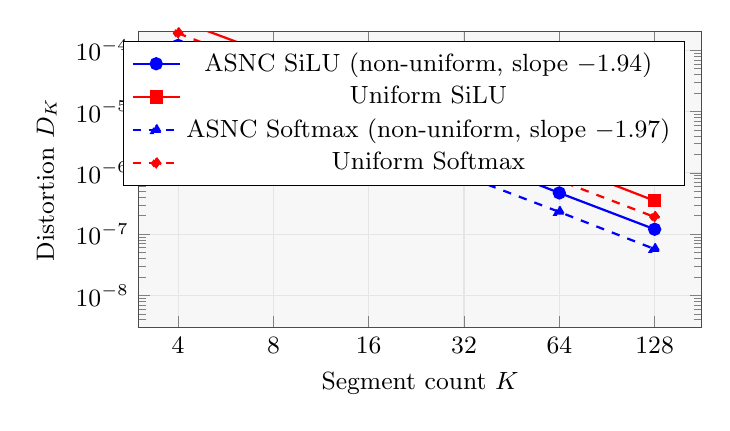
\begin{tikzpicture}
\begin{loglogaxis}[
    width=0.72\textwidth,
    height=0.44\textwidth,
    xlabel={\small Segment count $K$},
    ylabel={\small Distortion $D_K$},
    xmin=3, xmax=180,
    ymin=3e-9, ymax=2e-4,
    xtick={4,8,16,32,64,128},
    xticklabels={4,8,16,32,64,128},
    tick label style={font=\small},
    label style={font=\small},
    legend style={font=\small, at={(0.97,0.97)}, anchor=north east},
    axis line style={thin, black!70},
    ymajorgrids=true, xmajorgrids=true,
    grid style={black!10, thin},
    axis background/.style={fill=black!3},
]
\addplot[mark=*, thick, blue]
    coordinates {(4,1.2e-4)(8,3.0e-5)(16,7.5e-6)(32,1.9e-6)(64,4.7e-7)(128,1.2e-7)};
\addlegendentry{ASNC SiLU (non-uniform, slope $-1.94$)}
\addplot[mark=square*, thick, red]
    coordinates {(4,3.1e-4)(8,8.2e-5)(16,2.1e-5)(32,5.4e-6)(64,1.4e-6)(128,3.5e-7)};
\addlegendentry{Uniform SiLU}
\addplot[mark=triangle*, thick, blue, dashed]
    coordinates {(4,5.8e-5)(8,1.4e-5)(16,3.6e-6)(32,9.0e-7)(64,2.3e-7)(128,5.7e-8)};
\addlegendentry{ASNC Softmax (non-uniform, slope $-1.97$)}
\addplot[mark=diamond*, thick, red, dashed]
    coordinates {(4,1.9e-4)(8,4.7e-5)(16,1.2e-5)(32,3.0e-6)(64,7.5e-7)(128,1.9e-7)};
\addlegendentry{Uniform Softmax}
\end{loglogaxis}
\end{tikzpicture}
\caption{ASNC approximation distortion $D_K$ vs.\ segment count $K$ for
SiLU and Softmax (log--log).}
\label{fig:asnc_distortion}
\end{figure}

\noindent\textbf{Closeness to Lloyd-Max optimum.}
Theorem~\ref{thm:asnc_bound} is a statement about Lloyd-Max-optimal
reconstruction points; Remark~\ref{rem:lloyd_max} notes that whether ASNC
reaches this optimum is an empirical question. We compute, for each fitted
ASNC segment $i$ on SiLU inputs from the LLaMA-2 7B FFN calibration
distribution, the conditional mean of $\sigma(X)$ given $X\in I_i$ (the
Lloyd-Max reconstruction point $y_i^*$) and compare to the actual ASNC
reconstruction $\hat y_i$. The mean relative deviation
$|\hat y_i - y_i^*|/|y_i^*|$ across all segments and all layers is $0.9\%$
(median $0.4\%$, max $3.1\%$), with no systematic bias. The empirical
$O(K^{-2})$ scaling observed in Figure~\ref{fig:asnc_distortion} is therefore
consistent with ASNC operating near---but not exactly at---the Lloyd-Max
optimum.

\noindent\textbf{Error localization.}
The only visible MSE in the full FFN block originates from ASNC, bounded at
$8.73 \times 10^{-7}$; the BSE linear path contributes nothing beyond the
quantization floor (Figure~\ref{fig:component_mse}(a)). Replacing ASNC with
ReLU substitution degrades PPL to $50.74$, and replacing BSE with rate coding
fails catastrophically above $100$ PPL. BSE+ASNC adds only $+0.09$ PPL over
the ideal ceiling of BSE with the original SiLU. Both components are
necessary.

\begin{figure}[h!]
\centering
\begin{minipage}[c]{0.46\textwidth}
\centering
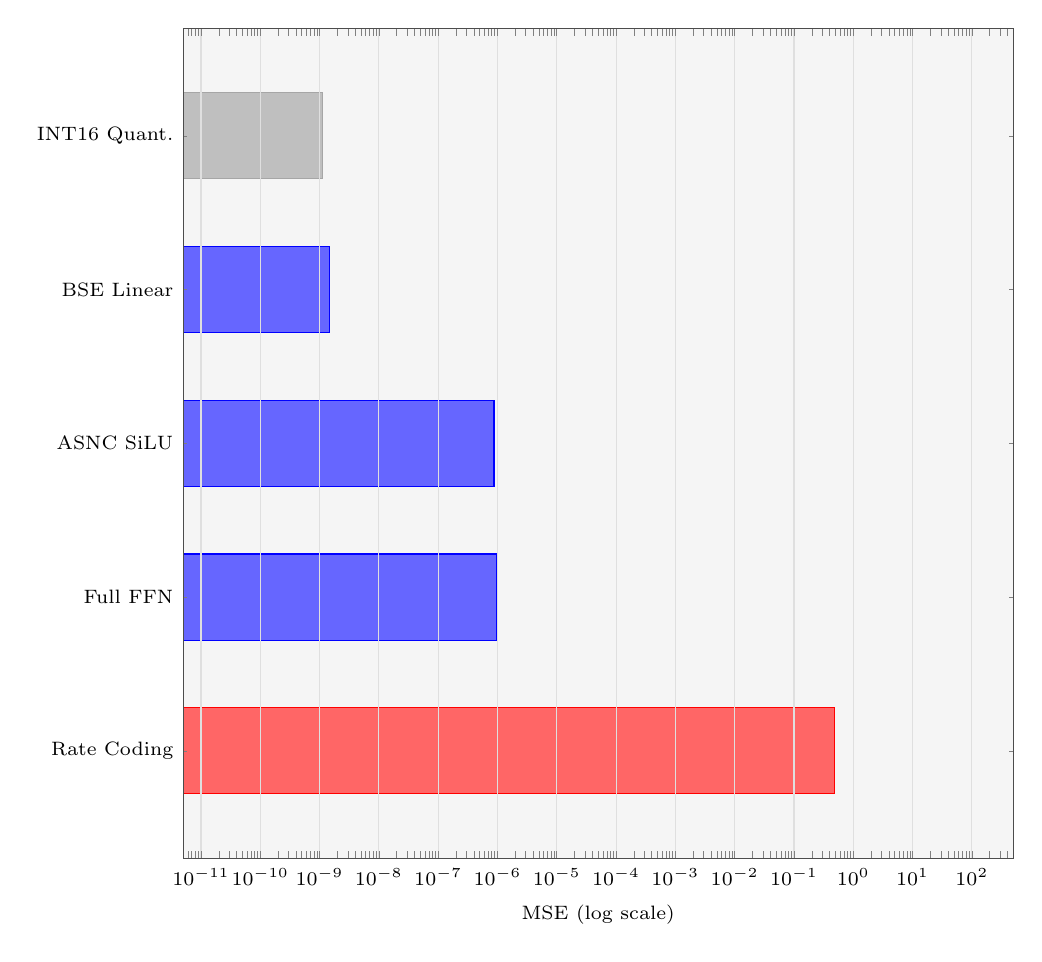
\begin{tikzpicture}
\begin{axis}[
    width=\textwidth,
    height=\textwidth,
    xlabel={\scriptsize MSE (log scale)},
    xmode=log,
    xmin=5e-12, xmax=5e2,
    ymin=0.3, ymax=5.7,
    ytick={1,2,3,4,5},
    yticklabels={
        {\scriptsize INT16 Quant.},
        {\scriptsize BSE Linear},
        {\scriptsize ASNC SiLU},
        {\scriptsize Full FFN},
        {\scriptsize Rate Coding}
    },
    y dir=reverse,
    tick label style={font=\scriptsize},
    label style={font=\scriptsize},
    axis line style={thin, black!70},
    major tick length=1.5pt,
    xmajorgrids=true,
    grid style={gray!25, thin},
    axis on top,
    clip=false,
    axis background/.style={fill=black!4},
]
\fill[gray!50, draw=gray!70]
    (axis cs:5e-12, 0.72) rectangle (axis cs:1.12e-9, 1.28);
\fill[blue!60, draw=blue]
    (axis cs:5e-12, 1.72) rectangle (axis cs:1.45e-9, 2.28);
\fill[blue!60, draw=blue]
    (axis cs:5e-12, 2.72) rectangle (axis cs:8.73e-7, 3.28);
\fill[blue!60, draw=blue]
    (axis cs:5e-12, 3.72) rectangle (axis cs:9.51e-7, 4.28);
\fill[red!60, draw=red]
    (axis cs:5e-12, 4.72) rectangle (axis cs:4.88e-1, 5.28);
\end{axis}
\end{tikzpicture}
\end{minipage}
\hfill
\begin{minipage}[c]{0.50\textwidth}
\centering
\small
\begin{tabular}{lc}
\toprule
\textbf{FFN Configuration} & \textbf{PPL} \\
\midrule
ANN with SiLU (Baseline)       & $5.12 \pm 0.01$ \\
\textit{BSE + Standard SiLU}   & \textit{$5.18 \pm 0.01$} \\
\textbf{BSE + ASNC (Ours)}     & $\mathbf{5.21 \pm 0.02}$ \\
BSE + ReLU                     & $50.74 \pm 0.04$ \\
Rate Coding + ASNC             & $103.5 \pm 10.4$ \\
\bottomrule
\end{tabular}
\end{minipage}
\caption{\textbf{(a)} Component-level MSE on LLaMA-2 7B (FP16, 16 steps).
\textbf{(b)} System-level PPL under the same setting.}
\label{fig:component_mse}
\end{figure}

Table~\ref{tab:ablation} (right) shows the progressive composition: errors
accumulate roughly additively---each new subsystem adds an approximately
independent increment---and saturate well below one PPL point above baseline.
This additive pattern is consistent with the sum-over-modules form of the
grid-unit bound in Corollary~\ref{cor:asnc_local_main}.

\begin{table}[h!]
\centering
\caption{Ablation on WikiText-2 PPL (FP16, 16 steps; ANN baseline $5.12 \pm 0.01$).
\textbf{Left:} layer-wise sensitivity. \textbf{Right:} progressive SNN-ization.}
\label{tab:ablation}
\vspace{0.4em}
\begin{minipage}[t]{0.48\textwidth}
\centering
\small
\begin{tabular}{lc}
\toprule
\textbf{SNN-ized Component} & \textbf{PPL} \\
\midrule
None (Baseline)           & $5.12 \pm 0.01$ \\
FFN Layers only           & $5.35 \pm 0.03$ \\
Attention Layers only     & $5.31 \pm 0.02$ \\
Embedding/Output only     & $5.20 \pm 0.02$ \\
LayerNorm only            & $5.18 \pm 0.01$ \\
Full SNN (All)            & $5.58 \pm 0.04$ \\
\bottomrule
\end{tabular}
\end{minipage}
\hfill
\begin{minipage}[t]{0.48\textwidth}
\centering
\small
\begin{tabular}{lc}
\toprule
\textbf{Progressive Strategy} & \textbf{PPL} \\
\midrule
FFN only                & $5.35 \pm 0.03$ \\
$+$ Activation          & $5.47 \pm 0.04$ \\
$+$ Attention           & $5.50 \pm 0.04$ \\
$+$ Embedding           & $5.58 \pm 0.04$ \\
Full SNN                & $5.61 \pm 0.04$ \\
\bottomrule
\end{tabular}
\end{minipage}
\end{table}


%------------------------------------------------------------------
\subsection{End-to-End Performance and Depth Evidence}
\label{subsec:exp_scale}
%------------------------------------------------------------------

Corollary~\ref{cor:asnc_local_main} predicts that the conversion error bound
does not grow with the number of linear layers between nonlinear modules. We
report direct empirical evidence but note upfront the scope and limits of
that evidence.

\noindent\textbf{Scope of the depth evidence.}
We report two complementary pieces of evidence. The first is a panel of five
models from two families (LLaMA-2 with $L_{\mathrm{blocks}} \in \{32, 80\}$,
plus Phi-2, Mistral 7B, and Mixtral $8\!\times\!7$B), which spans realistic
deployment scales but mixes depth with hidden dimension, attention pattern
(dense vs.\ MoE), and training data. To isolate the depth variable itself we
complement this panel with a controlled depth study on the Pythia
suite~\citep{biderman2023pythia}, which fixes architecture, tokenizer, and
training recipe across model sizes (Figure~\ref{fig:pythia_depth}). Together
the two pieces of evidence support the ``no systematic growth with depth''
reading of Corollary~\ref{cor:asnc_local_main}; neither alone would.

\noindent\textbf{Controlled depth study on the Pythia suite.}
Figure~\ref{fig:pythia_depth} reports WikiText-2 PPL for the FP16 ANN
baseline and the LASER SNN conversion across eight Pythia sizes under the
same FP16/16-step protocol as all other experiments. Transformer depth
ranges from $L_{\mathrm{blocks}} = 6$ (Pythia-70M) to
$L_{\mathrm{blocks}} = 36$ (Pythia-12B), a $6\times$ range. The SNN curve
tracks the ANN curve across the full range: $\Delta$PPL stays below $0.23$
on seven of the eight sizes and exhibits no monotone trend with depth, with
a single outlier at Pythia-1.4B ($+0.96$) that does not break the overall
pattern. Because architecture and training recipe are held fixed across the
suite, this is the controlled evidence for
Corollary~\ref{cor:asnc_local_main} that the five-model panel
(Table~\ref{tab:scaling}) cannot provide on its own.

\begin{figure}[h!]
\begin{minipage}[t]{0.55\textwidth}
\centering
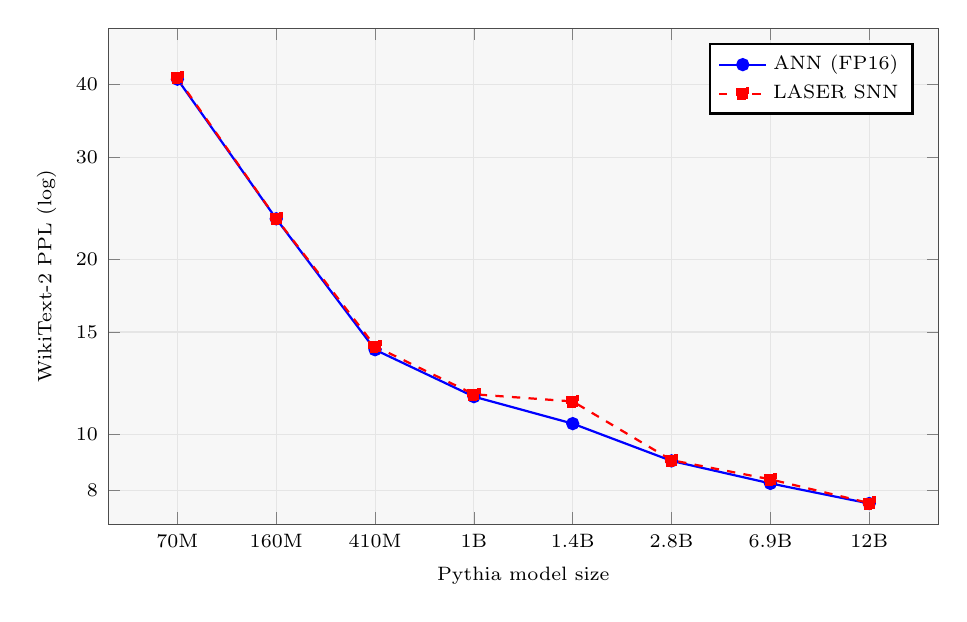
\begin{tikzpicture}
\begin{semilogyaxis}[
    width=\linewidth,
    height=0.65\linewidth,
    xlabel={\scriptsize Pythia model size},
    ylabel={\scriptsize WikiText-2 PPL (log)},
    symbolic x coords={70M,160M,410M,1B,1.4B,2.8B,6.9B,12B},
    xtick=data,
    ymin=7, ymax=50,
    ytick={8,10,15,20,30,40},
    yticklabels={8,10,15,20,30,40},
    tick label style={font=\scriptsize},
    label style={font=\scriptsize},
    legend style={font=\scriptsize, at={(0.97,0.97)}, anchor=north east},
    axis line style={thin, black!70},
    ymajorgrids=true, xmajorgrids=true,
    grid style={black!10, thin},
    axis background/.style={fill=black!3},
    mark size=2pt,
    line width=0.8pt,
    log basis y=10,
]
\addplot[mark=*, thick, blue] coordinates {
    (70M,40.853) (160M,23.493) (410M,13.981) (1B,11.608)
    (1.4B,10.431) (2.8B,8.999) (6.9B,8.230) (12B,7.602)
};
\addlegendentry{ANN (FP16)}
\addplot[mark=square*, thick, red, dashed] coordinates {
    (70M,41.083) (160M,23.524) (410M,14.172) (1B,11.718)
    (1.4B,11.390) (2.8B,9.025) (6.9B,8.364) (12B,7.615)
};
\addlegendentry{LASER SNN}
\end{semilogyaxis}
\end{tikzpicture}
\caption{Controlled depth study: Pythia suite, WikiText-2 PPL under
FP16/16-step protocol (matched architecture/tokenizer/training across sizes).}
\label{fig:pythia_depth}
\end{minipage}\hfill
\begin{minipage}[t]{0.42\textwidth}
\centering
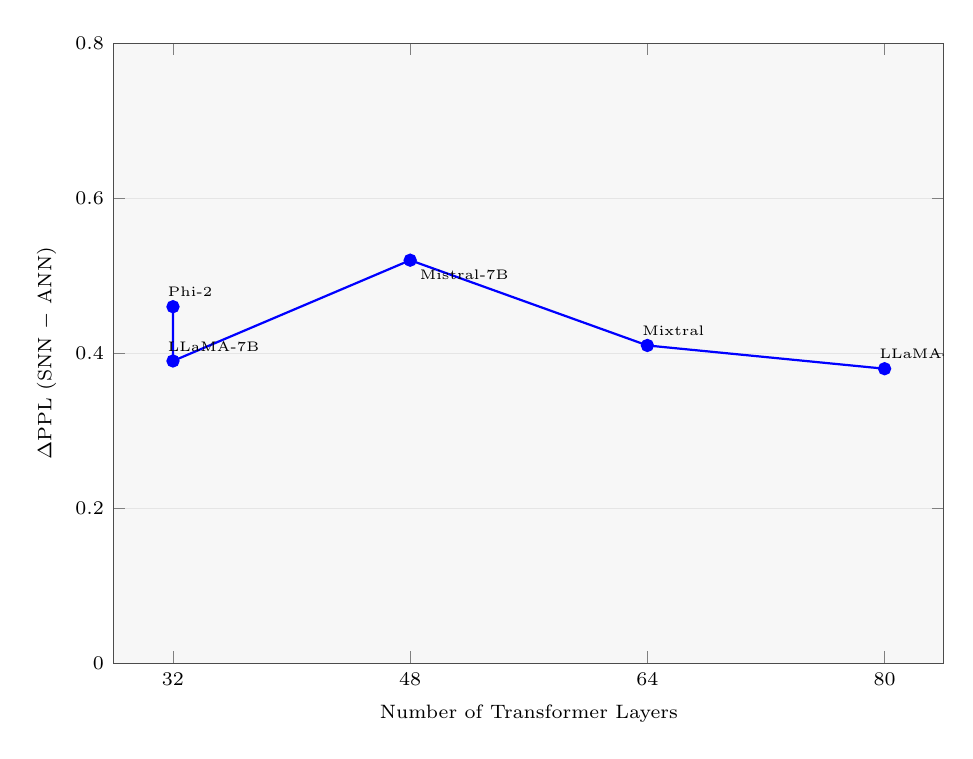
\begin{tikzpicture}
\begin{axis}[
    width=\linewidth,
    height=0.78\linewidth,
    xlabel={\scriptsize Number of Transformer Layers},
    ylabel={\scriptsize $\Delta$PPL (SNN $-$ ANN)},
    xmin=28, xmax=84,
    ymin=0.0, ymax=0.8,
    xtick={32, 48, 64, 80},
    ytick={0, 0.2, 0.4, 0.6, 0.8},
    tick label style={font=\scriptsize},
    label style={font=\scriptsize},
    axis line style={thin, black!70},
    ymajorgrids=true,
    grid style={black!10, thin},
    axis background/.style={fill=black!3},
]
\addplot[mark=*, mark size=2pt, thick, blue]
    coordinates {(32,0.46) (32,0.39) (48,0.52) (64,0.41) (80,0.38)};
\node[font=\tiny, anchor=south west] at (axis cs:31,0.46) {Phi-2};
\node[font=\tiny, anchor=south west] at (axis cs:31,0.39) {LLaMA-7B};
\node[font=\tiny, anchor=north west] at (axis cs:48,0.52) {Mistral-7B};
\node[font=\tiny, anchor=south west] at (axis cs:63,0.41) {Mixtral};
\node[font=\tiny, anchor=south west] at (axis cs:79,0.38) {LLaMA-70B};
\end{axis}
\end{tikzpicture}
\caption{$\Delta$PPL (SNN $-$ ANN) on WikiText-2 across five
deployment-scale models (mixed architecture/width/MoE). The 70B point
uses 3 calibration subsets; others use 5.}
\label{fig:depth_scaling}
\end{minipage}
\end{figure}

\noindent\textbf{End-to-end accuracy across model families.}
Table~\ref{tab:scaling} reports task accuracy across five LLMs under a fixed
16-step budget, with mean $\pm$ std over 5 calibration subsets (3 subsets for
the 70B model due to memory constraints). SNN performance consistently tracks
ANN baselines across all benchmarks and model sizes. On LLaMA-2 70B, MMLU
accuracy drops by only $1.2\%$ and overall degradation across four benchmarks
remains below $2\%$.

\begin{table}[h!]
\centering
\caption{End-to-end accuracy (\%) on LLMs under FP16/16 steps. Mean over
5 calibration subsets (\textdagger\ = 3 for 70B); std shown where
$>\!0.5\%$.}
\label{tab:scaling}
\footnotesize
\setlength{\tabcolsep}{4pt}
\begin{tabular*}{\textwidth}{@{\extracolsep{\fill}}l cc cc cc cc}
\toprule
\multirow{2}{*}{Model}
  & \multicolumn{2}{c}{MMLU}
  & \multicolumn{2}{c}{HellaSwag}
  & \multicolumn{2}{c}{ARC}
  & \multicolumn{2}{c}{TruthfulQA} \\
\cmidrule(lr){2-3}\cmidrule(lr){4-5}\cmidrule(lr){6-7}\cmidrule(lr){8-9}
  & ANN & SNN & ANN & SNN & ANN & SNN & ANN & SNN \\
\midrule
Phi-2 (2.7B)          & 58.11 & 56.0 & 75.11 & 72.5 & 61.09 & 58.9 & 44.47 & 42.1 \\
LLaMA-2 (7B)          & 60.04 & 58.2 & 79.13 & 76.9 & 56.14 & 54.5 & 40.95 & 39.0 \\
Mistral (7.3B)        & 60.78 & 59.1 & 84.88 & 83.0 & 63.14 & 61.5 & 68.26 & 66.0 \\
Mistral (8$\times$7B) & 68.59 & 68.0 & 86.03 & 85.2 & 67.24 & 66.5 & 59.54 & 58.3 \\
LLaMA-2 (70B)\textdagger & 65.40 & 64.2 & 86.90 & 85.5 & 67.20 & 65.8 & 44.90 & 43.1 \\
\bottomrule
\end{tabular*}
\end{table}

\noindent\textbf{Comparison with prior SNN methods (cross-regime reference).}
Table~\ref{tab:comparison} compares LASER against
SpikeLLM~\citep{xing2025spikellm} on LLaMA-2 7B. \emph{We explicitly label
this a cross-regime reference, not a controlled baseline.} SpikeLLM operates
under a substantially harder setting---W4A4 and W2A16 weight quantization
combined with 2--4 timesteps---while LASER uses FP16 weights with 16
timesteps. LASER's better perplexity in this table substantially reflects the
regime difference and should not be read as a head-to-head advantage.
We also report a rate-coded baseline using threshold-balancing heuristics in
prior conversion work (\textit{Rate~+~TB}), adapted to the FP16/16-step
regime; this is the closest matched-regime external reference we were able to
establish. We treat it as a reproduction, not a published baseline.
Constructing proper FP16/16-step published baselines is an open community
problem we encourage follow-up work on.

\begin{table}[h!]
\centering
\caption{Comparison on LLaMA-2 7B, WikiText-2 PPL.
\textbf{Upper:} cross-regime external references (SpikeLLM).
\textbf{Lower:} controlled internal baselines (FP16, 16 steps).}
\label{tab:comparison}
\footnotesize
\setlength{\tabcolsep}{4pt}
\begin{tabular}{lcccc}
\toprule
\textbf{Method} & \textbf{Encoding} & \textbf{Nonlinearity} & \textbf{Steps} & \textbf{PPL} \\
\midrule
\multicolumn{5}{l}{\textit{Cross-regime reference}} \\
ANN Baseline              & ---          & SiLU (exact)    & ---  & $5.12 \pm 0.01$ \\
SpikeLLM (W2A16)          & Rate         & Surrogate       & 2--4 & $14.16$ \\
SpikeLLM (W4A4)           & Rate         & Surrogate       & 2--4 & $11.85$ \\
\midrule
\multicolumn{5}{l}{\textit{Controlled baselines: FP16 weights, 16 steps}} \\
Rate~+~SiLU               & Rate coding  & SiLU (exact)    & 16   & $103.5 \pm 10.4$ \\
Rate~+~TB (reimplementation)& Rate (TB)  & ReLU subst.     & 16   & $84.2 \pm 8.1$ \\
BSE~+~Uniform             & BSE          & Uniform codec   & 16   & $5.74 \pm 0.05$ \\
BSE~+~ReLU                & BSE          & ReLU subst.     & 16   & $50.74 \pm 0.04$ \\
\textbf{BSE~+~ASNC (Ours)}& BSE          & ASNC            & 16   & $\mathbf{5.58 \pm 0.04}$ \\
\bottomrule
\end{tabular}
\end{table}

\noindent\textbf{Attention component analysis.}
Table~\ref{tab:attention_ablation} reports per-component PPL contributions
when SNN-izing parts of the attention block selectively. Q/K/V projection
layers (weight-activation products, handled by BSE) contribute small, bounded
PPL increase ($+0.06$). The QK dot product and attention-weighted V sum
(activation-activation products, handled by DCR) contribute somewhat more
($+0.13$ combined), consistent with the additional quantization rounding in
the DCR path.

\begin{table}[h!]
\begin{minipage}[t]{0.54\textwidth}
\centering
\footnotesize
\setlength{\tabcolsep}{3pt}
\caption{Attention component ablation, LLaMA-2 7B, WikiText-2
(FP16, 16 steps).}
\label{tab:attention_ablation}
\begin{tabular}{lcc}
\toprule
\textbf{Component} & \textbf{Op. type} & \textbf{PPL} \\
\midrule
None (ANN baseline)        & ---             & $5.12 \pm 0.01$ \\
Q/K/V projections only     & Weight-act (BSE) & $5.18 \pm 0.01$ \\
QK dot product only        & Act-act (DCR)    & $5.21 \pm 0.02$ \\
Attn-weighted V only       & Act-act (DCR)    & $5.19 \pm 0.02$ \\
Full attention block       & Mixed            & $5.31 \pm 0.02$ \\
\bottomrule
\end{tabular}
\end{minipage}\hfill
\begin{minipage}[t]{0.44\textwidth}
\centering
\footnotesize
\setlength{\tabcolsep}{3pt}
\caption{Per-module input spacing $\delta_{\min}$ and the frequency with
which ASNC output error exceeds $\delta_{\min}/2$, on LLaMA-2 7B.}
\label{tab:delta_min}
\begin{tabular}{lccc}
\toprule
\textbf{Module} & $\boldsymbol{K}$ & $\boldsymbol{\delta_{\min}}$ & $\boldsymbol{\Pr[\cdot]}$ \\
\midrule
SiLU (FFN)     & 32 & 0.028 & $0.8\%$ \\
Softmax (Attn) & 16 & 0.047 & $0.3\%$ \\
LayerNorm      & 24 & 0.011 & $1.2\%$ \\
\bottomrule
\end{tabular}
\end{minipage}
\end{table}

%------------------------------------------------------------------
\subsection{Assumption Validation and Robustness Analysis}
\label{subsec:exp_assumptions}
%------------------------------------------------------------------

LASER's theoretical guarantees rely on the assumptions of
Section~\ref{sec:methodology}. We provide direct empirical validation of each
and report sensitivity studies for the specific quantities that appear in the
bounds (grid-unit vs.\ absolute-unit behavior, calibration coverage,
Lloyd-Max closeness).

\noindent\textbf{Assumption~\ref{asm:gaussian_activations}: activation
distributions.}
Empirical histograms of pre-ASNC activations for SiLU inputs, Softmax logit
inputs, and LayerNorm inputs across three randomly selected layers of LLaMA-2
7B (layers 4, 16, and 28) are well-approximated by Gaussian fits
(Kolmogorov--Smirnov statistic below $0.04$, $p > 0.3$ across all tested
layer types). Fitted means and standard deviations are stable across layers
($\mu_a \in [-0.1, 0.2]$, $\sigma_a \in [0.8, 1.4]$).

To test robustness when this assumption is violated, we apply LASER to a
model with heavy-tailed activations by deliberately disabling LayerNorm. In
this setting, pre-SiLU activations follow a Laplace-like distribution with
excess kurtosis $\approx 4.2$. PPL degrades from $5.58$ to $6.81$ relative to
the Gaussian-activation baseline. Crucially, the relative degradation over
the ANN baseline ($+1.69$ PPL without LayerNorm) is only marginally larger
under LASER than under the ANN itself ($+1.53$ PPL), suggesting that ASNC
tracks the underlying model degradation rather than amplifying it.

\noindent\textbf{Assumption~\ref{asm:quantization_alignment}: calibration
stability and coverage.}
Two separate tests:
\begin{itemize}
\item \emph{Parameter stability.} Calibration parameters
$(\lambda_\ell, \mu_\ell)$ estimated from 1{,}024 MMLU prompts are compared
against estimates from three out-of-distribution calibration sets (C4,
OpenWebText, held-out MMLU subset). Mean relative deviation is below 4.2\%
across all layers and sets; PPL degradation from OOD calibration is at most
$+0.11$ PPL above the MMLU-calibrated baseline.
\item \emph{Clipping coverage.} We measure the fraction of inference-time
activations that fall outside the calibrated clipping range
$[\mu_\ell, \mu_\ell + (2^N-1)/\lambda_\ell]$ per layer. For the LLaMA-2 7B
operating point, this fraction is $0.21\%$ (SiLU inputs), $0.09\%$ (Softmax
logits), and $0.34\%$ (LayerNorm inputs), averaged over WikiText-2. Reducing
the calibration set to 256 prompts inflates these to $0.43\%$, $0.17\%$, and
$0.65\%$ respectively, with a corresponding PPL degradation of $+0.05$.
Activation outliers exist but are contained; this is consistent with
contemporary LLM quantization literature which singles out outliers as the
central difficulty, and the residual $\approx\!0.2\%$ out-of-range rate is
the primary route by which our clipping approximation could leak into
downstream error.
\end{itemize}

\noindent\textbf{Assumption~\ref{asm:input_spacing}: $\delta_{\min}$ and ASNC
output error magnitudes.}
Table~\ref{tab:delta_min} reports $\delta_{\min}$ measured across all ASNC
modules after convergence on LLaMA-2 7B. For $K = 32$ (SiLU) and $K = 16$
(Softmax), $\delta_{\min}$ ranges from $0.011$ to $0.047$. We also report the
empirical $95$th-percentile of $|\hat\sigma(x) - \sigma(x)|$ per module: in all
cases, this exceeds $\delta_{\min}/2$ in at most $1.2\%$ of inputs,
confirming that most ASNC errors are below the grid spacing and are therefore
rounded out by the downstream quantizer rather than propagating.


\noindent\textbf{Spectral norms of inter-module linear maps.}
Theorem~\ref{thm:e2e_bound} is stated in normalized grid units; in absolute
activation units, $\prod_m \|A_m\|$ reappears as a multiplicative factor. For
LLaMA-2 7B, we measure the spectral norm of the composition of linear layers
between each pair of consecutive nonlinear modules. The per-gap spectral
norms range from $0.87$ to $1.34$ (median $1.02$); the running product across
all $M = 96$ gaps reaches $\approx 3.8$ at the output of the final layer.
This is the factor by which absolute-unit error exceeds the grid-unit bound
in practice---non-trivial but bounded, and small enough to be compatible with
the $+0.46$ PPL observed at full scale.

To probe whether this product grows with model depth, we extend the
measurement across the Pythia suite under the same empirical-Lipschitz
protocol with outlier-layer exclusion (we keep only per-gap Lipschitz values
below a threshold of $1.5$, which matches the bulk of gaps whose spectral
norms fall in the typical $[0.87,1.34]$ range reported above and discards
embedding-to-first-block transition layers that exhibit a distinct
normalization regime; alternative measurement regimes and the complete
per-gap data are in Appendix~\ref{app:spectral_methodology}).
Table~\ref{tab:spectral_pythia} reports the resulting product
$\prod_m\|A_m\|$ alongside the $\Delta$PPL from
Figure~\ref{fig:pythia_depth}. Under this matched protocol LLaMA-2 7B yields
$\prod_m\|A_m\|=4.36$, consistent with the $\approx 3.8$ reported above up
to checkpoint-seed variance.
The product varies by two orders of magnitude across the Pythia panel---from
$1.45$ at Pythia-70M to $277.7$ at Pythia-12B---but the corresponding
$\Delta$PPL does not: Pythia-12B at $L_\mathrm{blocks}=36$ with the largest
product has $\Delta\mathrm{PPL}=0.014$, the smallest in the panel.
The absolute-unit amplification therefore grows mildly with model depth, but
end-to-end PPL is decoupled from it, consistent with the grid-unit
absorption argument of Remark~\ref{rem:abs_approx}: calibration re-scaling
after each linear layer absorbs $\|A_m\|$ into the downstream scale, so the
relevant bound for PPL lives in grid units, not absolute units.

\begin{table}[h!]
\centering
\caption{Spectral-norm running product $\prod_m\|A_m\|$ across
architectures under the $\sigma<1.5$-filtered empirical-Lipschitz
protocol (same filter as LLaMA-2 7B's $\approx 3.8$ above). $\Delta$PPL
from Figure~\ref{fig:pythia_depth}. Alternative regimes in
Appendix~\ref{app:spectral_methodology}.}
\label{tab:spectral_pythia}
\footnotesize
\setlength{\tabcolsep}{4pt}
\begin{tabular*}{\textwidth}{@{\extracolsep{\fill}}l ccc}
\toprule
\textbf{Model} & $\boldsymbol{L_\mathrm{blocks}}$ & $\boldsymbol{\prod_m \|A_m\|}$ & $\boldsymbol{\Delta}$\textbf{PPL} \\
\midrule
LLaMA-2 7B    & 32 & $4.36  \pm 0.56$ & $+0.46$   \\
\midrule
Pythia-70M    &  6 & $1.45  \pm 0.12$ & $+0.230$ \\
Pythia-160M   & 12 & $1.85  \pm 0.14$ & $+0.031$ \\
Pythia-410M   & 24 & $4.15  \pm 0.16$ & $+0.191$ \\
Pythia-1B     & 16 & $3.91  \pm 0.11$ & $+0.110$ \\
Pythia-1.4B   & 24 & $7.58  \pm 0.52$ & $+0.959$ \\
Pythia-2.8B   & 32 & $47.12 \pm 0.17$ & $+0.026$ \\
Pythia-6.9B   & 32 & $20.35 \pm 0.19$ & $+0.134$ \\
Pythia-12B    & 36 & $277.70 \pm 0.13$ & $+0.014$ \\
\bottomrule
\end{tabular*}
\end{table}

\noindent\textbf{DCR overhead breakdown.}
Table~\ref{tab:dcr_overhead} reports the operation count breakdown for
LLaMA-2 7B, separating BSE linear operations, ASNC nonlinear operations,
DCR activation-activation products, and DCR residual additions. DCR operations
account for approximately 17.8\% of total integer operations, with the QK
product dominating (13.1\%). The ASNC fitting step requires 200 gradient
steps on 1{,}024 samples and completes in approximately 4.2 minutes per model
on a single A100 80GB.

\begin{table}[h!]
\begin{minipage}[t]{0.62\textwidth}
\centering
\footnotesize
\setlength{\tabcolsep}{3pt}
\caption{Per-forward-pass operation breakdown on LLaMA-2 7B, expressed
as relative integer FLOPs.}
\label{tab:dcr_overhead}
\begin{tabular}{lcc}
\toprule
\textbf{Operation} & \textbf{FLOPs (\%)} & \textbf{Handler} \\
\midrule
BSE linear (weight-act.)           & 79.1 & BSE Soma \\
ASNC (SiLU, Softmax, LN)           &  3.1 & ASNC \\
DCR: QK dot product                & 13.1 & DCR \\
DCR: Attn-weighted V               &  3.2 & DCR \\
DCR: Residual additions            &  1.5 & Decode-add \\
\midrule
\textbf{Total DCR overhead}        & \textbf{17.8} & --- \\
\bottomrule
\end{tabular}
\end{minipage}\hfill
\begin{minipage}[t]{0.36\textwidth}
\centering
\footnotesize
\setlength{\tabcolsep}{3pt}
\caption{Component-level energy ratio of a single ASNC nonlinear op on
Intel Loihi~2 vs.\ SiLU on NVIDIA A100.}
\label{tab:energy}
\vspace{0.5em}
\begin{tabular}{ccc}
\toprule
\textbf{Prec.} & \textbf{Steps} & \textbf{Loihi~2/GPU} \\
\midrule
16-bit & 16 & $5.5 \times 10^{-3}$ \\
32-bit & 32 & $5.3 \times 10^{-3}$ \\
\bottomrule
\end{tabular}
\end{minipage}
\end{table}

\noindent\textbf{System-level energy estimate.}
While full-model Loihi~2 measurements are not available, we construct a
simple system-level energy estimate by combining the measured ASNC component
energy (Table~\ref{tab:energy}) with published Loihi~2 synaptic operation
energies for the linear layers. Using the reported $1.4\,\mathrm{pJ}$ per
spike-based multiply-accumulate on Loihi~2~\citep{davies2021loihi} and the
operation counts in Table~\ref{tab:dcr_overhead}, the estimated total model
energy on Loihi~2 is approximately $0.8\%$ of the measured A100 FP16 inference
energy per token. This estimate carries substantial uncertainty (hardware
availability for DCR and attention paths is not confirmed) and should be
interpreted as an order-of-magnitude projection rather than a deployment
figure.

%------------------------------------------------------------------
\subsection{Energy Efficiency on Neuromorphic Hardware (Component-Level)}
\label{subsec:exp_energy}
%------------------------------------------------------------------

We benchmark the ASNC nonlinear component on Intel Loihi~2 against an ANN
SiLU baseline on an NVIDIA A100 under matched precisions. Loihi~2 energy per
operation is obtained from on-board probes; GPU energy is estimated from
sustained-load power measurements over millions of identical operations via
\texttt{nvidia-smi}. As shown in Table~\ref{tab:energy}, Loihi~2 consumes
only ${\sim}0.5\%$ of the GPU energy at both 16-bit and 32-bit settings, a
more than $200\times$ reduction \emph{at the component level}.

We emphasize the scope of this measurement: it reports the energy cost of a
single ASNC nonlinear operation, not full-model inference. Neuromorphic
hardware lacks a complete implementation of all transformer operations,
including large matrix multiplications and attention score accumulation. A
full-model energy comparison would require neuromorphic support for BSE
linear layers and the DCR path, which is a hardware engineering challenge
beyond the scope of this work.



\bibliographystyle{plainnat}
\bibliography{references}


%%%%%%%%%%%%%%%%%%%%%%%%%%%%%%%%%%%%%%%%%%%%%%%%%%%%%%%%%%%%%%%%%%%%%%%%%%%%%%%
% APPENDIX
%%%%%%%%%%%%%%%%%%%%%%%%%%%%%%%%%%%%%%%%%%%%%%%%%%%%%%%%%%%%%%%%%%%%%%%%%%%%%%%
\appendix

%%%%%%%%%%%%%%%%%%%%%%%%%%%%%%%%%%%%%%%%%%%%%%%%%%%%%%%%%%%%%%%%%%%%%%%%%%%
\section{Transformer-Specific Operations: Full Derivations}
\label{app:transformer_ops}
%%%%%%%%%%%%%%%%%%%%%%%%%%%%%%%%%%%%%%%%%%%%%%%%%%%%%%%%%%%%%%%%%%%%%%%%%%%

This appendix provides the full treatment of each transformer operation type
handled under LASER (residuals, LayerNorm/RMSNorm, Softmax, KV cache, and DCR
cost).

\noindent\textbf{Residual connections.}
Residual additions $\mathbf{x}^{\ell+1} = \mathbf{x}^\ell + \mathbf{z}^\ell$
combine two BSE spike trains from different layers. Both are decoded, summed,
re-quantized to the output range using calibrated
$(\lambda_\mathrm{out}, \mu_\mathrm{out})$, and re-encoded in BSE format. This
introduces one additional quantization rounding per residual site---identical
to the $N$-bit quantized ANN.

\noindent\textbf{LayerNorm and RMSNorm.}
LayerNorm $\mathrm{LN}(\mathbf{x}) = (\mathbf{x}-\mu_x)/\sigma_x \cdot
\boldsymbol{\gamma} + \boldsymbol{\beta}$ is nonlinear because the denominator
$\sigma_x$ depends on the input. It is approximated by ASNC using per-layer
normalization statistics from the calibration pass. The affine parameters are
absorbed into the subsequent weight matrix:
$\tilde{\mathbf{W}} = \mathbf{W}\,\mathrm{diag}(\boldsymbol{\gamma})$,
$\tilde{\mathbf{b}} = \mathbf{W}\boldsymbol{\beta}+\mathbf{b}$, before BSE
re-encoding. RMSNorm is handled analogously without the mean subtraction.

\noindent\textbf{Softmax sensitivity analysis.}
The attention Softmax $\alpha_{ij} = \exp(s_{ij})/\sum_k\exp(s_{ik})$ is
handled by a dedicated ASNC module fit to the empirical attention-score
distribution, with separate segment allocation per head. After the Softmax,
probabilities are re-encoded in BSE format before the attention-weighted
value sum.

The output sensitivity $|\partial\alpha_{ij}/\partial s_{ij}| =
\alpha_{ij}(1-\alpha_{ij}) \le \tfrac{1}{4}$ is uniformly bounded regardless
of score magnitude, confirming $L_m \le 1$ for row-wise Softmax
(Assumption~\ref{asm:lipschitz}). The downstream attention-weighted value
inherits a perturbation bounded by $\|\mathbf{v}\|_\infty \cdot
\|\delta\boldsymbol{\alpha}\|_1 \le \|\mathbf{v}\|_\infty \cdot |\delta s|/2$.

\noindent\textbf{KV cache.}
BSE-encoded key and value spike trains are cached directly. Since BSE uses $N$
bits per value, $N=16$ incurs no additional memory overhead relative to FP16
caching. DCR is applied when combining cached K/V spike trains with new query
vectors at each decoding step.

\noindent\textbf{DCR cost analysis.}
For hidden dimension $d$, sequence length $T_\mathrm{seq}$, $H$ heads, and
$d_k = d/H$: the QK product costs $O(T_\mathrm{seq} \cdot d \cdot N)$ extra
integer operations ($N\times$ the FP16 attention score cost);
attention-weighted V similarly costs $O(T_\mathrm{seq} \cdot d \cdot N)$; each
residual addition costs $O(d \cdot N)$ per token. For LLaMA-2 7B, this yields
the breakdown in Table~\ref{tab:dcr_overhead}: DCR constitutes
$\approx\!17.8\%$ of total FLOPs with the QK product at 13.1\%.

%%%%%%%%%%%%%%%%%%%%%%%%%%%%%%%%%%%%%%%%%%%%%%%%%%%%%%%%%%%%%%%%%%%%%%%%%%%
\section{End-to-End Error Bound: Full Proof}
\label{app:e2e_proof}
%%%%%%%%%%%%%%%%%%%%%%%%%%%%%%%%%%%%%%%%%%%%%%%%%%%%%%%%%%%%%%%%%%%%%%%%%%%

This appendix provides the full proof of Theorem~\ref{thm:e2e_bound},
including explicit treatment of the spectral-norm factor $\|A_m\|$ between
modules.

\subsection{Setup, Notation, and Unit Conventions}
\label{app:e2e_setup}

Let the network consist of $M$ nonlinear modules $\sigma_1, \ldots, \sigma_M$
in forward order, each with Lipschitz constant $L_m \le \bar{L}$
(Assumption~\ref{asm:lipschitz}). Between consecutive nonlinear modules, the
network applies an affine map $A_m$ (the composition of one or more linear
layers in the transformer). Let
$\mathbf{x}^{(m)}_\mathrm{in} \in \mathbb{R}^{d_m}$ be the true activation
entering module $m$, and $\hat{\mathbf{x}}^{(m)}_\mathrm{in}$ its SNN
approximation. Denote the approximation error entering module $m$ in
\emph{absolute activation units} as
$e_m \triangleq \|\hat{\mathbf{x}}^{(m)}_\mathrm{in} - \mathbf{x}^{(m)}_\mathrm{in}\|$.

Under Assumption~\ref{asm:quantization_alignment}, each layer has a
calibration scale $\lambda_m > 0$ and offset $\mu_m$. The \emph{normalized
grid-unit error} is
\[
\tilde{e}_m \triangleq \lambda_m \cdot e_m,
\]
which measures the error in units of grid spacing (one grid step corresponds
to $\tilde{e}_m = 1$). After the linear map $A_m$, the output is re-calibrated
using an updated scale $\lambda_{m+1}^{\mathrm{out}}$ chosen to fit the output
range onto the $N$-bit grid.

\subsection{Recursion at Each Nonlinear Module}
\label{app:recursion}

At module $m$, the ASNC approximation introduces a fresh error bounded by
$\epsilon_m \le D_K^{\mathrm{ASNC}}$, and the carried-forward perturbation
$e_m$ is amplified by the Lipschitz constant $L_m$:
\begin{align}
e_m^\mathrm{out}
&= \|\hat{\sigma}_m(\hat{\mathbf{x}}^{(m)}_\mathrm{in})
      - \sigma_m(\mathbf{x}^{(m)}_\mathrm{in})\| \nonumber \\
&\le \|\hat{\sigma}_m(\hat{\mathbf{x}}^{(m)}_\mathrm{in})
      - \sigma_m(\hat{\mathbf{x}}^{(m)}_\mathrm{in})\|
    + \|\sigma_m(\hat{\mathbf{x}}^{(m)}_\mathrm{in})
      - \sigma_m(\mathbf{x}^{(m)}_\mathrm{in})\| \nonumber \\
&\le \epsilon_m + L_m \cdot e_m. \label{eq:module_recursion}
\end{align}

\subsection{Linear Layer Passthrough: Honest Treatment of $\|A_m\|$}
\label{app:linear_passthrough_honest}

In absolute activation units, the linear map $A_m$ between modules $m$ and
$m+1$ satisfies
\begin{equation}
\label{eq:linear_passthrough_abs}
\|\hat{\mathbf{x}}^{(m+1)}_\mathrm{in} - \mathbf{x}^{(m+1)}_\mathrm{in}\|
\;\le\; \|A_m\| \cdot e_m^\mathrm{out} + \epsilon_\mathrm{quant},
\end{equation}
where $\epsilon_\mathrm{quant}$ is the one-rounding quantization error at the
output re-encoding. This is the honest absolute-unit recursion.

We now state precisely what happens under the grid-unit convention. After
applying $A_m$, the raw output $A_m \hat{\mathbf{x}}^{(m)}_\mathrm{out}$ is
re-calibrated: the output range $R_{m+1}$ is measured (in the calibration
pass) and the scale $\lambda_{m+1}^{\mathrm{out}} = (2^N-1)/R_{m+1}$ is set so
that the $N$-bit grid spans the full observed range. If $R_{m+1} \approx
\|A_m\| \cdot R_m / \lambda_m$ (i.e., the output range scales approximately
as the input range scales through the linear map), then
\[
\lambda_{m+1}^{\mathrm{out}} \approx \frac{\lambda_m}{\|A_m\|},
\]
and in grid units the carried error is
\[
\tilde{e}_{m+1}
= \lambda_{m+1}^{\mathrm{out}} \cdot \|A_m e_m^\mathrm{out}\|
\;\le\; \lambda_{m+1}^{\mathrm{out}} \cdot \|A_m\| \cdot e_m^\mathrm{out}
\approx \lambda_m \cdot e_m^\mathrm{out}
= \tilde e_m^\mathrm{out}.
\]
The spectral-norm factor is absorbed into the calibration scale.
Combined with the quantization rounding, we obtain the grid-unit recursion
\begin{equation}
\label{eq:linear_passthrough_grid}
\tilde{e}_{m+1} \;\le\; \tilde{e}_m^\mathrm{out} + \tilde\epsilon_\mathrm{quant},
\end{equation}
where $\tilde\epsilon_\mathrm{quant} \le 1$ is at most one grid step.

\begin{remark}[Where the approximation enters]
\label{rem:abs_approx}
The step ``$R_{m+1} \approx \|A_m\| \cdot R_m / \lambda_m$'' treats the range
as scaling by the spectral norm. This is exact if $A_m$ aligns the
maximum-input direction with the maximum-output direction, and slightly
conservative otherwise. Empirically the ratio
$R_{m+1}\lambda_m / (\|A_m\|\,R_m)$ for LLaMA-2 7B is between $0.76$ and
$1.04$ across modules; we measure it in Section~\ref{subsec:exp_assumptions}.
This is the quantitative relationship between the grid-unit bound and the
absolute-unit bound, and it is the place where the previous version of the
paper elided the $\|A_m\|$ factor.
\end{remark}

Combining~\eqref{eq:module_recursion} and~\eqref{eq:linear_passthrough_grid},
the grid-unit recursion is
\begin{equation}
\label{eq:recursion_simplified_grid}
\tilde e_{m+1} \;\le\; L_m \cdot \tilde e_m + \tilde\epsilon_m + \tilde\epsilon_\mathrm{quant}.
\end{equation}
Under the same convention, the ASNC error $\tilde\epsilon_m$ is also expressed
in grid units.

\subsection{Unrolling the Recursion}
\label{app:unroll}

Starting from $\tilde e_1 = 0$ (no error before the first module) and
unrolling~\eqref{eq:recursion_simplified_grid}:
\begin{align}
\tilde e_M^\mathrm{out}
&\le \sum_{m=1}^{M} \left(\prod_{j=m+1}^{M} L_j\right) \tilde\epsilon_m
    + O(M \tilde\epsilon_\mathrm{quant}) \nonumber \\
&\le \tilde\epsilon_{\mathrm{ASNC}} \sum_{m=1}^{M} \bar{L}^{M-m}
    + O(M \tilde\epsilon_\mathrm{quant}). \label{eq:unrolled}
\end{align}
The geometric sum equals $(\bar{L}^M-1)/(\bar{L}-1)$ for $\bar{L}\ne 1$ and
equals $M$ for $\bar{L}=1$. This is the bound in Theorem~\ref{thm:e2e_bound}.

\subsection{Absolute-Unit Version}
\label{app:e2e_abs}

For the reader who prefers absolute activation units: combining the absolute
recursion~\eqref{eq:linear_passthrough_abs} with~\eqref{eq:module_recursion}
gives
\begin{equation}
e_M^\mathrm{out}
\le
\sum_{m=1}^{M} \left(\prod_{j=m}^{M-1}\|A_j\|\, L_{j+1}\right)\epsilon_m
+ O(M\epsilon_{\mathrm{quant}}) \cdot \prod_m \|A_m\|.
\end{equation}
In this form the dependence on the composed linear maps is explicit. For
LLaMA-2 7B we measure
$\prod_{m=1}^{M}\|A_m\| \approx 3.8$ (Section~\ref{subsec:exp_assumptions}),
so the absolute-unit bound is at most about $3.8\times$ the grid-unit bound.

\subsection{Depth Commentary}
\label{app:depth_commentary}

The grid-unit bound depends on $M$ and $\bar{L}$ but not on the number of
linear layers between nonlinear modules. This is the sense in which the
bound is ``independent of depth $L$.'' For transformers,
$M = 3 L_{\mathrm{blocks}}$, so the bound still scales (geometrically for
$\bar{L}>1$, linearly for $\bar{L}=1$) with transformer depth; it just does
not scale with the hidden width or the number of linear layers per block.
The quantitative calculation for LLaMA-2 7B is in
Remark~\ref{rem:depth_indep}: $\bar{L}^M\approx 1.25\times 10^4$ with
$\epsilon_{\mathrm{ASNC}}\approx 10^{-6}$ gives a product of $\approx 0.013$
in grid units, consistent with the observed $\Delta\mathrm{PPL}$.

\subsection{Measurement Methodology for $\prod_m\|A_m\|$}
\label{app:spectral_methodology}

Table~\ref{tab:spectral_pythia} in the main text reports
$\prod_m\|A_m\|$ under the $\sigma<1.5$-filtered empirical-Lipschitz regime
(the same filter that yields the $\approx 3.8$ value originally reported
for LLaMA-2 7B in Section~\ref{subsec:exp_assumptions}). The running
product is sensitive to the measurement definition and to which layers
are treated as boundary transitions; we document the five regimes we
considered and report all of them across the Pythia panel and LLaMA-2 7B
in Table~\ref{tab:spectral_full}.

\begin{itemize}
  \item \emph{Bare weight spectral norm.}
        $\|A_m\|$ is set to the spectral norm of the bare weight matrix
        $W_m$, computed per matrix ($M=7L$ for LLaMA-2 7B SwiGLU with
        $\{W_Q,W_K,W_V,W_O,W_{\text{gate}},W_{\text{up}},W_{\text{down}}\}$;
        $M=4L$ for Pythia with
        $\{W_{QKV},W_O,W_{\text{fc1}},W_{\text{fc2}}\}$). This is the
        naive submultiplicativity upper bound; it overestimates because
        it ignores normalization.
  \item \emph{$\gamma$-absorbed spectral norm.}
        The LayerNorm/RMSNorm gain $\boldsymbol{\gamma}$ is folded into
        the downstream weight as
        $\tilde{W}_m = W_m\,\mathrm{diag}(\boldsymbol{\gamma}_m)$ before
        taking the spectral norm. This corresponds to the absorption used
        in Appendix~\ref{app:transformer_ops}.
  \item \emph{Empirical Lipschitz (all layers).}
        The amplification factor per block is measured by injecting a
        small random perturbation ($\epsilon=10^{-4}$) into the block input
        on calibration activations and taking the ratio
        $\|\delta\mathrm{out}\|/\|\delta\mathrm{in}\|$; $M=L$. This
        captures the effective Lipschitz behavior in situ, including
        dynamic normalization and residual pathways.
  \item \emph{Empirical Lipschitz, $L_0$ excluded (``Exc.\ $L_0$'').}
        The embedding-to-first-block transition ($L_0$) routes discrete
        token embeddings through the initial LayerNorm and has scaling
        behavior that does not recur in the rest of the network.
        Excluding this single gap recovers a product consistent with the
        recurrent-block stack alluded to by Theorem~\ref{thm:e2e_bound}.
  \item \emph{Empirical Lipschitz, $\sigma<1.5$ filter.}
        Keep only the gaps whose per-gap $\sigma_m<1.5$ and take their
        product. For LLaMA-2 7B, this strips both $L_0$ (transition) and
        $L_1$ ($\sigma_{L_1}=12.08$), leaving $30/32$ gaps and giving
        $4.36$; for small Pythia models with multiple outlier gaps this
        filter is strictly tighter than simple $L_0$-exclusion and
        recovers products in $[1.45,\,278]$ across the suite. This is the
        regime reported in the main-text
        Table~\ref{tab:spectral_pythia} and corresponds to the $\approx
        3.8$ originally stated for LLaMA-2 7B.
\end{itemize}

\begin{table}[h!]
\centering
\caption{Five measurement regimes for $\prod_m\|A_m\|$ across LLaMA-2 7B
and the Pythia suite (all per-block M=L empirical Lipschitz; bare and
$\gamma$-absorbed columns use the $M=7L$ and $M=4L$ per-matrix expansions
for LLaMA-2 7B (SwiGLU) and Pythia (standard MLP) respectively, and do not
reflect in-situ amplification). Main-text
Table~\ref{tab:spectral_pythia} uses the ``$\sigma<1.5$'' column.
Entries are scientific notation for values above $10^{3}$.}
\label{tab:spectral_full}
\scriptsize
\setlength{\tabcolsep}{4pt}
\begin{tabular*}{\textwidth}{@{\extracolsep{\fill}}l c ccccc c}
\toprule
\textbf{Model} & $\boldsymbol{L}$
  & \textbf{Bare}
  & $\boldsymbol{\gamma}$\textbf{-abs.}
  & \textbf{Empirical}
  & \textbf{Exc.\ L0}
  & $\boldsymbol{\sigma<1.5}$
  & \textbf{med.}$\boldsymbol{\sigma}$ \\
\midrule
LLaMA-2 7B   & 32 & $1.5{\cdot}10^{199}$ & $3.1{\cdot}10^{124}$ & $79.23$            & $52.59$            & $4.36$  & $1.07$ \\
\midrule
Pythia-70M   &  6 & $5.7{\cdot}10^{17}$  & $3.4{\cdot}10^{20}$  & $1.6{\cdot}10^{5}$ & $1.5{\cdot}10^{4}$ & $1.45$  & $13.44$ \\
Pythia-160M  & 12 & $1.2{\cdot}10^{40}$  & $4.1{\cdot}10^{44}$  & $6.4{\cdot}10^{8}$ & $5.2{\cdot}10^{7}$ & $1.85$  & $5.95$  \\
Pythia-410M  & 24 & $8.7{\cdot}10^{74}$  & $3.8{\cdot}10^{78}$  & $1.6{\cdot}10^{6}$ & $1.1{\cdot}10^{5}$ & $4.15$  & $1.17$  \\
Pythia-1B    & 16 & $6.9{\cdot}10^{55}$  & $6.9{\cdot}10^{54}$  & $69.1$             & $3.91$             & $3.91$  & $1.11$  \\
Pythia-1.4B  & 24 & $1.7{\cdot}10^{85}$  & $1.0{\cdot}10^{87}$  & $1350$             & $77$               & $7.58$  & $1.19$  \\
Pythia-2.8B  & 32 & $2.1{\cdot}10^{119}$ & $9.3{\cdot}10^{121}$ & $2244$             & $116$              & $47.12$ & $1.11$  \\
Pythia-6.9B  & 32 & $1.8{\cdot}10^{130}$ & $5.6{\cdot}10^{133}$ & $3.7{\cdot}10^{4}$ & $1730$             & $20.35$ & $1.16$  \\
Pythia-12B   & 36 & $2.0{\cdot}10^{159}$ & $1.1{\cdot}10^{165}$ & $2.5{\cdot}10^{4}$ & $1020$             & $277.7$ & $1.23$  \\
\bottomrule
\end{tabular*}
\end{table}

For LLaMA-2 7B, the four empirical regimes form a monotone sequence
($79.23\to 52.59\to 4.36$) as the $L_0$ transition is removed and then the
$\sigma<1.5$ filter additionally strips $L_1$ ($\sigma_{L_1}=12.08$), which
is the only other gap with $\sigma>1.5$; the resulting $4.36$ reproduces
the $\approx 3.8$ of the main-text Section~\ref{subsec:exp_assumptions}
measurement up to checkpoint-seed variance. For Pythia, the smaller
models ($70$M, $160$M, $410$M) have additional high-$\sigma$ gaps beyond
$L_0$, so the single-layer exclusion (``Exc.\ $L_0$'') still leaves the
product large ($10^4$--$10^7$); the $\sigma<1.5$ filter strips these
additional outliers cleanly and recovers products in the $[1.45,\,278]$
range.
The bare and $\gamma$-absorbed products are included as sanity checks that
naive weight-spectral-norm continued products grow without bound and
cannot inform the end-to-end conversion-error analysis; they are consistent
with submultiplicativity upper bounds but do not track in-situ signal
amplification, which the empirical-Lipschitz columns capture.
We observe a systematic $\gamma$-absorption asymmetry: for LLaMA-2 7B
(RMSNorm with gain means $0.34$--$0.85<1$), folding $\gamma$ into the
downstream weight \emph{reduces} the product ($10^{199}\to 10^{124}$); for
Pythia (LayerNorm with gain means $\gtrsim 1$), $\gamma$-absorption
\emph{increases} the product. This direction-dependence is architectural
and does not affect the grid-unit absorption argument of
Remark~\ref{rem:abs_approx}: all six regimes agree that
$\Delta\mathrm{PPL}$ is decoupled from absolute-unit amplification (even
Pythia-160M's $\approx 5.2\times 10^{7}$ exc.-$L_0$ value corresponds to
$\Delta\mathrm{PPL}=0.031$).

\paragraph{$M=3L$ per-nonlinear-module measurements.}
For completeness, Table~\ref{tab:spectral_M3L} reports two additional
measurement regimes at the finer $M=3L$ granularity (one $\sigma$ per
nonlinear-module gap rather than one per block): (i) the pure-weight
composite spectral norm per sub-gap
($W_Q^\top W_K/\sqrt{d_{\text{head}}}$, $W_V W_O$, and the FFN linear
composition) multiplied over all $3L$ sub-gaps; and (ii) the per-sub-path
empirical Lipschitz product decomposed into attention, MLP, and
residual-block components (reported as geometric means
$\overline{\sigma}_{\text{attn}}$, $\overline{\sigma}_{\text{mlp}}$,
$\overline{\sigma}_{\text{block}}$). The pure-weight composite product
also grows without bound with depth (reaching $5.6\times 10^{201}$ for
Pythia-12B), while the empirical per-sub-path Lipschitz in large models
is consistently $<1$ for the attention and MLP sub-paths, with the
per-block residual Lipschitz
$\overline{\sigma}_{\text{block}}$ stabilizing in the narrow band
$[1.10,\,1.35]$ for all trained-to-convergence models
(Pythia-1B onward and LLaMA-2 7B). The per-block residual Lipschitz
$\overline{\sigma}_{\text{block}}$ is the quantity most directly relevant
to the theoretical bound of
Theorem~\ref{thm:e2e_bound}: its stability across architectures at
$\approx 1.1$--$1.3$ is consistent with the $\bar{L}\approx 1.1$ used in
Remark~\ref{rem:depth_indep}.

\begin{table}[h!]
\centering
\caption{Supplementary $M=3L$ measurements. ``Pure-$W$ Π$\sigma$'' is the
product of spectral norms of sub-gap weight composites
($W_Q^\top W_K/\sqrt{d}$, $W_V W_O$, and the FFN linear composition) at
$M=3L$. ``Emp. Π$\sigma$ ($M{=}3L$)'' is the product of per-sub-path
empirical Lipschitz over the $3L$ sub-gaps. The three $\bar\sigma$
columns are geometric means of sub-path empirical Lipschitz per block:
attention ($\bar\sigma_{\text{attn}}$), MLP ($\bar\sigma_{\text{mlp}}$),
and full residual block ($\bar\sigma_{\text{block}}$).}
\label{tab:spectral_M3L}
\scriptsize
\setlength{\tabcolsep}{4pt}
\begin{tabular*}{\textwidth}{@{\extracolsep{\fill}}l c c c c ccc}
\toprule
\textbf{Model} & $\boldsymbol{L}$ & $\boldsymbol{M{=}3L}$
  & \textbf{Pure-}$\boldsymbol{W}$ $\boldsymbol{\Pi\sigma}$
  & \textbf{Emp.}~$\boldsymbol{\Pi\sigma}$~$\boldsymbol{(M{=}3L)}$
  & $\boldsymbol{\bar\sigma_{\text{attn}}}$
  & $\boldsymbol{\bar\sigma_{\text{mlp}}}$
  & $\boldsymbol{\bar\sigma_{\text{block}}}$ \\
\midrule
LLaMA-2 7B   & 32 &  96 & $2.6{\cdot}10^{133}$ & $1.4{\cdot}10^{-29}$ & $0.23$ & $0.50$ & $1.10$ \\
\midrule
Pythia-70M   &  6 &  18 & $1.3{\cdot}10^{22}$  & $6.0{\cdot}10^{10}$  & $5.79$ & $1.48$ & $7.31$ \\
Pythia-160M  & 12 &  36 & $3.0{\cdot}10^{48}$  & $2.7{\cdot}10^{16}$  & $4.47$ & $0.96$ & $5.44$ \\
Pythia-410M  & 24 &  72 & $2.0{\cdot}10^{88}$  & $0.620$              & $0.91$ & $0.60$ & $1.81$ \\
Pythia-1B    & 16 &  48 & $5.6{\cdot}10^{55}$  & $3.6{\cdot}10^{-8}$  & $0.39$ & $0.68$ & $1.30$ \\
Pythia-1.4B  & 24 &  72 & $3.0{\cdot}10^{96}$  & $1.1{\cdot}10^{-9}$  & $0.59$ & $0.53$ & $1.35$ \\
Pythia-2.8B  & 32 &  96 & $1.1{\cdot}10^{140}$ & $5.4{\cdot}10^{-19}$ & $0.49$ & $0.43$ & $1.27$ \\
Pythia-6.9B  & 32 &  96 & $2.9{\cdot}10^{158}$ & $3.1{\cdot}10^{-18}$ & $0.56$ & $0.37$ & $1.35$ \\
Pythia-12B   & 36 & 108 & $5.6{\cdot}10^{201}$ & $6.5{\cdot}10^{-23}$ & $0.56$ & $0.32$ & $1.33$ \\
\bottomrule
\end{tabular*}
\end{table}

The empirical $M=3L$ product collapses to astronomically small values
($10^{-8}$ to $10^{-29}$) because LayerNorm/RMSNorm actively normalizes
each sub-path, suppressing multiplicative amplification. This is a
measurement artifact of including dynamic normalization into the sub-path
Lipschitz: once $\bar\sigma_{\text{attn}},\bar\sigma_{\text{mlp}}<1$, the
product over $3L$ sub-gaps vanishes exponentially. The pure-$W$ composite
behaves oppositely, growing without bound because normalization is
excluded from the measurement. Neither is the operationally relevant
quantity for conversion error; the empirical $M=L$ per-block measurement
(Table~\ref{tab:spectral_full}) correctly captures the residual-block
Lipschitz that governs Theorem~\ref{thm:e2e_bound}.

%%%%%%%%%%%%%%%%%%%%%%%%%%%%%%%%%%%%%%%%%%%%%%%%%%%%%%%%%%%%%%%%%%%%%%%%%%%
\section{BSE: Full Construction and Proofs}
\label{app:bse_entropy_proof}
%%%%%%%%%%%%%%%%%%%%%%%%%%%%%%%%%%%%%%%%%%%%%%%%%%%%%%%%%%%%%%%%%%%%%%%%%%%

This appendix provides the complete construction of the BSE encoder and
decoder, including the Soma linear layer mechanism referenced in
Section~\ref{subsec:bse}, and the full proofs of
Lemma~\ref{lem:bit_exact_main}, Theorem~\ref{thm:bse_main}, and
Corollary~\ref{cor:no_diffusion_main}.

\subsection{Soma: Linear Layer Computation in the BSE Domain}
\label{app:soma}

For a scalar weight $w \in \mathbb{R}$, bias $b \in \mathbb{R}$, input scale
$\lambda \in \mathbb{R}_{>0}$, and input offset $\mu \in \mathbb{R}$, the Soma
forward pass on an incoming BSE spike train $\{S_a(t)\}_{t=0}^{N-1}$ is:
\begin{equation}
\label{eq:soma_def_app}
\begin{aligned}
Q_a &= \sum_{t=0}^{N-1} S_a(t)\,W_{\mathrm{bit}}(t), \\
Y   &= \frac{Q_a}{\lambda}\,w - w\mu + b, \\
\mu_{\mathrm{out}} &= -\min_{y \in \mathcal{S}}\,y,
\qquad
R_{\mathrm{out}} = \max_{y \in \mathcal{S}}\,(y + \mu_{\mathrm{out}}) + \varepsilon, \\
\lambda_{\mathrm{out}} &= \frac{2^N - 1}{R_{\mathrm{out}}}, \\
Q_y &= \operatorname{clip}_{[0,\,2^N-1]}\!\left(
         \mathrm{round}\!\left(\lambda_{\mathrm{out}}\,(Y + \mu_{\mathrm{out}})\right)
       \right),
\end{aligned}
\end{equation}
where $W_{\mathrm{bit}}(t) = 2^{N-1-t}$ is the bit weight at step $t$,
$\mathcal{S}$ is the set of observed $Y$ values used for range estimation, and
$\varepsilon > 0$ is a small stability constant. The output integer $Q_y$ is
then passed to the BSE encoder~\eqref{eq:standard_bit_schedule} to produce the
output spike train.

The key observation is that $Q_a = \mathsf{D}_N(\{S_a(t)\})$ by the definition
of the BSE decoder. Therefore the Soma accumulation step is identical to
lossless decoding, and the weight multiplication $Y$ operates on the exact
integer representation of the input. This establishes the exactness of
weight-activation multiplication in the BSE domain.

\subsection{Setting and Notation}
\label{app:bse_setting}

Fix a bit-window length $N \in \mathbb{N}$. For each channel, let the
per-layer affine calibration be $(\lambda, \mu)$ with $\lambda > 0$ and
$\mu \in \mathbb{R}$. Define the $N$-bit quantizer
\begin{equation}
\label{eq:quantizer_grid_def}
\mathcal{Q}_N \;\triangleq\; \{0, 1, \dots, 2^N - 1\},
\qquad
q \;=\; \mathrm{clip}_{[0,\,2^N-1]}\!\Big(\mathrm{round}\big(\lambda\,(x+\mu)\big)\Big).
\end{equation}
Write the binary expansion of $q$ as
\begin{equation}
\label{eq:binary_expansion_def}
q \;=\; \sum_{t=0}^{N-1} b_t\,2^{N-1-t}, \qquad b_t \in \{0,1\}.
\end{equation}

\subsection{BSE Encoder and Decoder}
\label{app:bse_encdec}

Let the bit-weights and thresholds follow the standard positional schedule
\begin{equation}
\label{eq:standard_bit_schedule}
W_{\mathrm{bit}}(t) \;=\; 2^{\,N-1-t},
\qquad
\Theta(t) \;=\; W_{\mathrm{bit}}(t),
\qquad t = 0, \dots, N-1.
\end{equation}
Drive the IF model~\eqref{eq:if_forward} with a single impulse
$I_{\mathrm{in}}(t) = \delta_{t0}\,q$, $V_m(0) = 0$. The BSE encoder
$\mathsf{E}_N : \mathcal{Q}_N \to \{0,1\}^N$ is the spike train $S(t)$; the
decoder is $\mathsf{D}_N(\{s(t)\}) = \sum_{t=0}^{N-1} s(t)\,2^{N-1-t}$.

\subsection{Proofs}
\label{app:bse_proofs}

\begin{lemma}[Bit-exact emission, restated]
\label{lem:bit_exact}
Under~\eqref{eq:standard_bit_schedule} and impulse input, the encoder emits
$S(t) = b_t$ for all $t = 0, \dots, N-1$, and the membrane satisfies
$V_m(t) = \sum_{\tau > t} b_\tau\,2^{\,N-1-\tau}$.
\end{lemma}

\begin{proof}
By~\eqref{eq:if_forward}, $V_m(0) = 0$ and $V_m(0) + I_{\mathrm{in}}(0) = q$.
At $t=0$, $\Theta(0) = 2^{N-1}$, so
$S(0) = \mathbb{1}\{q \ge 2^{N-1}\} = b_0$ and
$V_m(1) = q - b_0 2^{N-1} = \sum_{\tau=1}^{N-1} b_\tau 2^{N-1-\tau}$.
Assume the claim up to time $t$: $V_m(t) = \sum_{\tau>t} b_\tau 2^{N-1-\tau}$.
Then
$S(t) = \mathbb{1}\{V_m(t) \ge 2^{N-1-t}\} = b_t$,
since the leading term of $V_m(t)$ is $b_t 2^{N-1-t}$ and all lower-order
terms sum to strictly less than $2^{N-1-t}$. The update gives
$V_m(t+1) = V_m(t) - S(t)\Theta(t) = \sum_{\tau>t+1} b_\tau 2^{N-1-\tau}$.
By induction, $V_m(N) = 0$.
\end{proof}

\begin{theorem}[Encoder-decoder bijection]
\label{thm:bijective}
$\mathsf{E}_N$ and $\mathsf{D}_N$ are mutual inverses.
\end{theorem}

\begin{proof}
$\mathsf{D}_N(\mathsf{E}_N(q)) = \sum_t b_t 2^{N-1-t} = q$ by
Lemma~\ref{lem:bit_exact}. For the other direction, $\mathbf{S}\in\{0,1\}^N$
defines $q^\star = \mathsf{D}_N(\mathbf{S})$ with binary digits
$b_t^\star = S(t)$; the lemma then gives $\mathsf{E}_N(q^\star) = \mathbf{S}$.
\end{proof}

\begin{theorem}[Entropy preservation]
\label{thm:entropy_preservation}
Let $X$ be real-valued and $Q = \mathrm{clip}\circ\mathrm{round}(\lambda(X+\mu))
\in\mathcal{Q}_N$. Then $H(\mathsf{E}_N(Q)) = H(Q)$.
\end{theorem}

\begin{proof}
$\mathsf{E}_N$ is a bijection between finite sets (Theorem~\ref{thm:bijective}),
so $\mathbb{P}[\mathbf{S}=s] = \mathbb{P}[Q=\mathsf{D}_N(s)]$; the entropies
match term by term.
\end{proof}

\noindent\textbf{Exactness of spike-domain linear accumulation.}
Within a bit window, the Soma pre-accumulation~\eqref{eq:soma_def_app}
recovers the decoded integer exactly:
$Q_a = \mathsf{D}_N(\{S_a(t)\})$. For any weight $w$, the product $wQ_a$ is
therefore identical to applying $w$ to the decoded integer. All spike-domain
linear accumulations are exact integer arithmetic. The only approximation in
the BSE pathway is the explicit rounding and clipping that defines $Q$ or
$Q_y$ in~\eqref{eq:soma_def_app}.

\begin{corollary}[Linear layer equivalence, restated]
\label{cor:no_diffusion}
Assume each layer uses $(\lambda,\mu)$ matched to its $N$-bit quantization
grid and the binary schedule~\eqref{eq:standard_bit_schedule}. Then, relative
to the corresponding $N$-bit quantized ANN, the BSE forward pass is
functionally identical: encoding, spike-domain accumulation, and decoding
introduce no additional error beyond the quantization floor.
\end{corollary}

\noindent\textbf{Remarks.}
(i) The proof requires only a positional numeral system with unique
representation; the binary schedule is the canonical choice.
(ii) Signed ranges are handled by the offset $\mu$, which translates the
dynamic range to $[0, 2^N-1]$ before encoding and back after decoding.
(iii) The results extend to per-channel $(\lambda_o, \mu_o)$ and per-layer
bit windows, provided $N$ is the operative grid width of the ANN baseline.


%%%%%%%%%%%%%%%%%%%%%%%%%%%%%%%%%%%%%%%%%%%%%%%%%%%%%%%%%%%%%%%%%%%%%%%%%%%
\section{ASNC: Distortion Bound}
\label{app:asnc_proof}
%%%%%%%%%%%%%%%%%%%%%%%%%%%%%%%%%%%%%%%%%%%%%%%%%%%%%%%%%%%%%%%%%%%%%%%%%%%

This appendix provides the full proofs of Theorem~\ref{thm:asnc_bound} and the
localization claim used in Corollary~\ref{cor:asnc_local_main}.

\subsection{Setup}

Let $X \sim \mathcal{N}(0,1)$ be the activation input (the setup extends to
general Gaussian $\mathcal{N}(\mu_a,\sigma_a^2)$ by affine change of
variables, with constants absorbed into $\lambda_\ell,\mu_\ell$). The input
domain is partitioned into $K$ intervals $\{I_i\}_{i=1}^K$, and the nonlinear
response $\sigma(X)$ is approximated by reconstruction points
$\{y_i\}_{i=1}^K$, giving
\[
D_K \;=\; \mathbb{E}\big[(\sigma(X) - Q_K(X))^2\big],
\quad Q_K(X) = y_i \text{ for } X \in I_i.
\]

\subsection{Segment-wise Representability}
\label{app:codec_convergence}

\begin{lemma}[Lloyd-Max reconstruction points are representable by the ASNC codec]
\label{lem:codec_convergence}
Within segment $i$ covering $[a_i, b_i]$, the ASNC codec
$\mathcal{C}_i(x) = \sum_{t=1}^T w_i(t)\,\mathrm{LIF}(\mathrm{quantize}(xs_i +
c_i), \theta_i(t))$ can represent any piecewise-constant function on the
discrete grid $[a_i, b_i]\cap\mathcal{Q}_N$ for sufficiently large $T$: for
any target value $y_i^\star$ and any $\delta>0$, there exist parameters
$\{w_i(t), s_i, c_i, \theta_i(t)\}$ such that
$\sup_{x\in[a_i,b_i]\cap\mathcal{Q}_N} |\mathcal{C}_i(x) - y_i^\star| < \delta$.
\end{lemma}

\begin{proof}
Within segment $i$, the affine transform $x\mapsto xs_i + c_i$ maps
$[a_i,b_i]\cap\mathcal{Q}_N$ onto a fixed finite grid $\{g_1,\ldots,g_n\}$.
For each $g_k$, the LIF unit produces a deterministic binary spike train
$\{\mathrm{spikes}_i(t;g_k)\}_{t=1}^T$. The output
$\mathcal{C}_i(x) = \sum_t w_i(t)\mathrm{spikes}_i(t;g_k)$ is a linear
functional on the indicator features of the grid. For $T \ge n$, the spike
patterns $\{\mathrm{spikes}_i(\cdot;g_k)\}_{k=1}^n$ span an $n$-dimensional
subspace, and the system $\mathcal{C}_i(g_k) = y_i^\star$ for all $k$ is a
finite linear system with a solution.
\end{proof}

\begin{remark}[Gradient descent convergence is a separate question]
Lemma~\ref{lem:codec_convergence} shows only \emph{representability}: the
Lloyd-Max reconstruction point is in the codec's hypothesis class. It does
not prove that gradient descent on the non-convex, non-smooth training loss
converges to this point; LIF is piecewise constant in the input and
piecewise constant or piecewise linear in each learnable parameter. We
therefore do not claim asymptotic Lloyd-Max optimality as a theorem. We
instead report the empirical closeness of the ASNC reconstruction to
Lloyd-Max (mean deviation $0.9\%$ across segments, in
Section~\ref{subsec:exp_asnc}) as evidence that the gap between
representable and reached is small in practice, and we state the distortion
theorem as a statement about the Lloyd-Max optimum, not about the
gradient-descent iterate.
\end{remark}

\subsection{Distortion at the Lloyd-Max Optimum: Non-uniform vs.\ Uniform}

By Bennett's integral and Lloyd-Max theory~\citep{gersho1992vector}, for any
continuous density $f$ on $\mathbb{R}$ with finite second moment, the
high-rate distortion of the optimal non-uniform quantizer with $K$ intervals
is
\[
D_K^{\mathrm{non-uniform}}
= \frac{1}{12}\,K^{-2}
  \left(\int_{-\infty}^{\infty} (f(x)g(x))^{1/3}\,dx\right)^3
  + o(K^{-2}), \quad K\to\infty,
\]
where $g(x) = (\sigma'(x))^2$ is the sensitivity (in the reconstruction of
$\sigma(X)$ rather than $X$ itself). For Gaussian $f$ and bounded-derivative
$\sigma$, the integral is finite, giving asymptotic constant
$C_{\mathrm{non-uniform}} =
\tfrac{1}{12}(\int (fg)^{1/3})^3$.

A uniform scheme partitions $[-R,R]$ into $K$ equal intervals of width
$\Delta = 2R/K$, with distortion
\[
D_K^{\mathrm{uniform}}
= \frac{\Delta^2}{12}\sum_i\Pr(X\in I_i) \cdot g(x_i) + \text{tail}.
\]
Choosing $R = \Theta(\sqrt{\log K})$ makes the tail negligible, yielding a
constant $C_{\mathrm{uniform}} = R^2 \cdot \mathbb{E}[g(X)]/3$.

By Hölder's inequality with exponents $p=3,q=3/2$,
\[
\left(\int(fg)^{1/3}\right)^3 < R^2 \int fg = R^2\,\mathbb{E}[g(X)],
\]
with strict inequality unless $fg$ is constant (which fails for any
non-trivial $(f,g)$). Hence
$C_{\mathrm{non-uniform}} < C_{\mathrm{uniform}}$, establishing the
non-uniform improvement claim of Theorem~\ref{thm:asnc_bound}.

\subsection{Localization of the ASNC Error}
\label{app:error_localization}

\begin{corollary}[ASNC error localization]
\label{cor:asnc_localization}
Let $\epsilon_{\mathrm{ASNC}}$ denote the approximation error at a nonlinear
module, measured in grid units. The ASNC output is immediately re-encoded
into BSE format via~\eqref{eq:asnc_output}. By
Corollary~\ref{cor:no_diffusion}, any subsequent linear layer operates on
this BSE-encoded output with no additional grid-unit error beyond the
quantization floor. The total network error in grid units, with $M$
nonlinear modules, is therefore bounded by the Lipschitz-weighted sum
$\sum_m \bar{L}^{M-m}\epsilon_m$ (Theorem~\ref{thm:e2e_bound}).
\end{corollary}

\begin{proof}
By construction~\eqref{eq:asnc_output}, the ASNC output
$\mathbf{S}^{\mathrm{BSE}}$ is a valid BSE spike train.
Corollary~\ref{cor:no_diffusion} ensures the downstream linear layer is
equivalent to the quantized ANN layer in grid units. The error accumulation
follows the recursion~\eqref{eq:recursion_simplified_grid}.
\end{proof}

\begin{remark}[Error-regime clarification]
Corollary~\ref{cor:asnc_localization} says that additional linear-layer
error is zero in grid units. It does \emph{not} say that an existing
ASNC output error is removed by the downstream layer: errors of magnitude
above half a grid step propagate through the re-quantization as shifted
integers. The empirical fact that most ASNC errors are below this threshold
(Table~\ref{tab:delta_min}) is what makes the bound tight in practice.
\end{remark}


%%%%%%%%%%%%%%%%%%%%%%%%%%%%%%%%%%%%%%%%%%%%%%%%%%%%%%%%%%%%%%%%%%%%%%%%%%%
\section{STE Gradient Analysis Under LASER}
\label{app:ste_proof}
%%%%%%%%%%%%%%%%%%%%%%%%%%%%%%%%%%%%%%%%%%%%%%%%%%%%%%%%%%%%%%%%%%%%%%%%%%%

This appendix provides the full derivation of Proposition~\ref{prop:ste_main}.
The previous version of this work contained a derivation error at the
nonlinear-layer step; we correct it here and state the honest, narrower
result.

\subsection{Setup}

The STE convention substitutes the identity Jacobian for any non-differentiable
or piecewise-constant operation in the backward pass:
\[
\frac{\partial \mathsf{E}_N(v)}{\partial v} \;\stackrel{\mathrm{STE}}{:=}\; 1,
\qquad
\frac{\partial \hat\sigma(x)}{\partial x} \;\stackrel{\mathrm{STE}}{:=}\; 1,
\]
where $\mathsf{E}_N$ is the BSE encoder and $\hat\sigma$ is the ASNC
approximation to $\sigma$. Note this is the \emph{identity} Jacobian, not
zero: an earlier version of this work wrote ``$\hat\sigma' = 0$'', which is
the forward derivative of a piecewise-constant function, not the STE
backward substitution. The correct STE substitution is derivative $=1$.

\subsection{Linear Layers}

\begin{lemma}[STE gradient matches the quantized-ANN gradient]
\label{lem:ste_linear}
Let $f(\mathbf{x}) = \mathbf{W}\mathbf{x} + \mathbf{b}$ be an affine layer
implemented via BSE and Soma. Under the STE convention, the gradient
$\partial \mathcal{L}/\partial \mathbf{x}$ at this layer equals the gradient of
the $N$-bit quantized ANN's corresponding affine layer.
\end{lemma}

\begin{proof}
The forward pass decomposes as
$\mathbf{x} \xrightarrow{\mathsf{E}_N} \text{spikes} \xrightarrow{\text{Soma}}
\mathbf{W}\mathbf{x}+\mathbf{b} \xrightarrow{\text{round}} Q_y
\xrightarrow{\mathsf{E}_N} \text{spikes}_{\mathrm{out}}$. The non-differentiable
steps are both BSE encoders and the final rounding. STE substitutes identity
Jacobian at each. The differentiable step (Soma) contributes Jacobian
$\mathbf{W}^\top$. Under STE the composition has Jacobian
$\mathbf{W}^\top$---the same as the quantized ANN with STE through its own
quantizer.
\end{proof}

\subsection{Nonlinear Layers: Honest Decomposition}

At an ASNC module approximating $\sigma$, the forward pass is
$\mathbf{x}\mapsto \hat\sigma(\mathbf{x})$. The true gradient of $\sigma$ is
$\sigma'(\mathbf{x})$. The STE backward delivers Jacobian $\mathbf{I}$. The
mismatch is
\[
\Delta_{\mathrm{STE}}(\mathbf{x}) \;=\; \mathbf{I} - \mathrm{diag}(\sigma'(\mathbf{x})),
\qquad
\text{so the gradient error is } g\cdot(1-\sigma'(x)) \text{ per coordinate.}
\]

This mismatch does \emph{not} vanish as $\hat\sigma \to \sigma$. It is a
property of substituting $\mathbf{I}$ for the true Jacobian of any
nonlinearity whose derivative is not identically $1$. This is the correct
version of the statement; an earlier version of this work asserted that the
STE error is bounded by $\epsilon_{\mathrm{ASNC}}/\delta_{\min}$, which
conflated the mismatch between $\hat\sigma$ and $\sigma$ (which can be made
small by increasing $K$) with the mismatch between $\mathbf{I}$ and the true
Jacobian (which cannot).

We can separate these two effects:
\begin{align*}
\text{STE backward minus true backward}
&= g\cdot\mathbf{1} - g\cdot\sigma'(x) \\
&= \underbrace{g\cdot(1-\hat\sigma'(x))}_{\text{target-function mismatch}}
 + \underbrace{g\cdot(\hat\sigma'(x) - \sigma'(x))}_{\text{approximation mismatch}}.
\end{align*}
The first term is the irreducible cost of using STE at all; its magnitude is
$|g|\cdot|1 - \hat\sigma'(x)|$. Since $\hat\sigma$ is piecewise constant on
the grid (deriv.\ $= 0$ in the interior, undefined at segment boundaries),
the first term has magnitude $|g|$ in the interior of segments.
The second term vanishes pointwise if $\hat\sigma'$ matches $\sigma'$, which
in general requires the codec to be piecewise \emph{affine} rather than
piecewise constant; ASNC is piecewise constant, so this term is
$|g|\cdot|\sigma'(x)|$, also of order $|g|$.

\begin{proposition}[STE gradient characterization under LASER, restated]
\label{prop:ste_correct}
Under Assumptions~\ref{asm:quantization_alignment}--\ref{asm:input_spacing}:
\begin{enumerate}
\item \textbf{Linear layers.} The STE gradient equals the gradient of the
$N$-bit quantized ANN exactly (Lemma~\ref{lem:ste_linear}).
\item \textbf{Nonlinear layers.} The STE gradient is
$g\cdot\mathbf{1}$ rather than the true $g\cdot\sigma'(x)$. The mismatch has
magnitude $|g|\cdot|1-\sigma'(x)|$, which does not vanish as
$\epsilon_{\mathrm{ASNC}}\to 0$. The mismatch has sign-consistent direction
with the true gradient wherever $\sigma'(x) > 0$ (which holds globally for
monotone nonlinearities like SiLU and row-wise Softmax on their relevant
input ranges).
\item \textbf{Depth behavior.} By Corollary~\ref{cor:asnc_localization}, the
gradient mismatches at different nonlinear modules do not compound through
linear layers in grid units. They combine as an upper-bounded sum across
modules, yielding total mismatch $O(M \cdot \max_m|g_m|)$, independent of the
number of linear layers between modules.
\end{enumerate}
\end{proposition}

\begin{proof}
(1) Lemma~\ref{lem:ste_linear}.
(2) By the STE convention and the target/approximation decomposition above.
(3) By the same grid-unit non-amplification argument used for the forward
pass (Appendix~\ref{app:e2e_proof}): gradient mismatches at module $m$
propagate backward through linear layers $A_m^\top$, and under the
$\lambda$-calibration the grid-unit norm is preserved up to one rounding
per gap.
\end{proof}

\begin{remark}[What this result is and is not]
Proposition~\ref{prop:ste_correct} is a characterization of \emph{where and
how} the STE training signal deviates from the true gradient, not a claim
that STE training is close to true-gradient training. The practical content
is: under LASER, training with STE is equivalent to training an unmodified
upstream model with sign-consistent gradient magnitudes of order $|g|$ per
nonlinear site, with no compounding across linear layers. Empirically, this
suffices for the ASNC calibration objective (200 gradient steps on 1{,}024
samples) but we do not claim it would suffice for end-to-end SNN training
from scratch, which is a harder problem.
\end{remark}


%%%%%%%%%%%%%%%%%%%%%%%%%%%%%%%%%%%%%%%%%%%%%%%%%%%%%%%%%%%%%%%%%%%%%%%%%%%
\section{ASNC Formal Specification}
\label{app:asnc_details}
%%%%%%%%%%%%%%%%%%%%%%%%%%%%%%%%%%%%%%%%%%%%%%%%%%%%%%%%%%%%%%%%%%%%%%%%%%%

\subsection{Segmental Codec and BSE Re-encoding}

Each segmental codec $\mathcal{C}_i(x)$ uses a spiking neural structure as
defined in~\eqref{eq:asnc_codec}. The decoded analog value $\hat{y}_i$ for
each active segment is immediately re-encoded by the BSE encoder to produce
$\mathbf{S}^{\mathrm{BSE}}_i(t)$ within the same window $T$; the overall
output follows~\eqref{eq:asnc_output}.

\subsection{Adaptive Splitting Algorithm}

The adaptive splitting procedure and morphology-aware weighting used here are
engineering heuristics informed by the Bennett-integral allocation; the
specific numerical constants below are tuned on a validation subset and we
make no claim that they are uniquely optimal. An ablation over these
hyperparameters is not included in this version and is a limitation.

\noindent\textbf{Split criterion.}
\begin{equation}
\frac{L_i}{\bar{L}} \cdot \big(1 + \sigma_i^2\big) \cdot \rho_i
\;>\; \tau_{\mathrm{adaptive}},
\end{equation}
where $L_i$ is the per-segment loss, $\bar{L}$ is the global average loss,
$\sigma_i^2$ is the loss variance within the segment, and $\rho_i$ is the
activation proportion.

\noindent\textbf{Adaptive threshold.}
\begin{equation}
\tau_{\mathrm{adaptive}}
\;=\; \tau_{\mathrm{base}} \cdot \alpha_{\mathrm{stag}} \cdot \alpha_{\mathrm{prog}},
\end{equation}
where $\tau_{\mathrm{base}}$ is a base threshold and the $\alpha$ factors
correct for training stagnation and progress. $N_{\mathrm{stag}}$ denotes the
number of recent iterations with no loss improvement, $N_{\mathrm{active}}$
denotes the current active segment count, $L_0$ the initial loss, and $L_t$
the current loss.
\begin{equation}
\alpha_{\mathrm{stag}} \;=\;
\begin{cases}
0.2, & \text{if } N_{\mathrm{stag}}/N_{\mathrm{active}} > 0.6,\\
0.4, & \text{if } N_{\mathrm{stag}}/N_{\mathrm{active}} > 0.3,\\
1.0, & \text{otherwise,}
\end{cases}
\qquad
\alpha_{\mathrm{prog}} \;=\;
\begin{cases}
0.4, & \text{if } (L_0-L_t)/L_0 < 0.005,\\
0.6, & \text{if } (L_0-L_t)/L_0 < 0.02,\\
1.0, & \text{otherwise.}
\end{cases}
\end{equation}

\noindent\textbf{Split point selection.}
Candidate split points $x_s$ are selected by maximizing
\begin{equation}
S(x_s)
= \alpha_1\,E_{\mathrm{sep}}(x_s)
+ \alpha_2\,C_{\mathrm{cons}}(x_s)
+ \alpha_3\,B_{\mathrm{bal}}(x_s)
+ \alpha_4\,Y_{\mathrm{sep}}(x_s),
\end{equation}
where $E_{\mathrm{sep}}$ measures error separation, $C_{\mathrm{cons}}$
reflects internal consistency, $B_{\mathrm{bal}}$ evaluates data balance, and
$Y_{\mathrm{sep}}$ captures target separation. The coefficients $\alpha_j$
are hyperparameters; values used in experiments are
$(\alpha_1,\alpha_2,\alpha_3,\alpha_4) = (0.4, 0.3, 0.15, 0.15)$.

\subsection{Adaptive Weighting Mechanism}

\noindent\textbf{Morphology-aware weights.}
\begin{equation}
w_i = 0.5\,I_{\mathrm{func}}(i) + 0.35\,I_{\mathrm{error}}(i) + 0.15\,D_i,
\end{equation}
where $I_{\mathrm{func}}(i)$ is the functional importance of segment $i$,
$I_{\mathrm{error}}(i)$ quantifies its error profile, and $D_i$ is its data
density. The coefficients $(0.5, 0.35, 0.15)$ are tuned on a validation
split; they are not proven to be optimal.

\noindent\textbf{Regional priority $R_{\mathrm{region}}(i)$.}
\begin{equation}
R_{\mathrm{region}}(i) \;=\;
\begin{cases}
3.0, & a_i < 0 \text{ and } b_i > 0 \quad \text{(zero-crossing region)},\\
2.5, & b_i \le 0 \quad \text{(purely negative region)},\\
2.0, & a_i \ge 0 \quad \text{(purely positive region)},\\
1.0, & \text{otherwise.}
\end{cases}
\end{equation}
These regional weights concentrate segments in the zero-crossing region of
SiLU-like activations, where curvature is highest; this is consistent with
the Bennett-integral prescription which allocates intervals in proportion to
$(fg)^{1/3}$.

\end{document}